\documentclass[10pt]{article}


%%%%%%%%%%%%%%%%%%%%%%%%%%%%%%%%%%%%%%%%%%%%%%%%%%%%%%%%%%%%%%%%%%%%%%%%%%%%%%%%%%%%%%
%%%%%%%%%%%%%%%%%%% YOU PROBABLY DON"T NEED TO CHANGE ANYTHING HERE %%%%%%%%%%%%%%%%%%%
\usepackage[numbers,sort]{natbib}
\usepackage{amsfonts, amsmath} 
\usepackage{graphicx}
\usepackage{libertine} 
\usepackage{fullpage}
\usepackage{hyperref}
\usepackage{cleveref}
\usepackage{subcaption}
\usepackage{placeins}
\hypersetup{
    colorlinks = true,
    linkcolor = blue,
    urlcolor  = blue,
    citecolor = blue,
    anchorcolor = blue}
\urlstyle{same}
%%%%%%%%%%%%%%%%%%%%%%%%%%%%%%%%%%%%%%%%%%%%%%%%%%%%%%%%%%%%%%%%%%%%%%%%%%%%%%%%%%%%%%
%%%%%%%%%%%%%%%%%%%%%%%%%%%%%%%%%%%%%%%%%%%%%%%%%%%%%%%%%%%%%%%%%%%%%%%%%%%%%%%%%%%%%%


%
% ===== DOCUMENT STARTS HERE =======
% you do not have to modify anything above
% if you do not wish to (but you indeed can0
%
\begin{document}

\title{Effects of Ambient Dimension and Active-Subspace Alignment on Bayesian Optimisation and CMA-ES }
\date{\today}
\maketitle

{\bf Group Composition:}
\begin{enumerate}
\item Seow Chuan Zheng, A0271623J, \href{mailto:e1121026@u.nus.edu}{e1121026@u.nus.edu}
\end{enumerate}

{\bf Github Repository:} \url{https://github.com/digreenycode/Bayesian-Project}


\section{Introduction}

Bayesian optimisation (BO) and CMA-ES take different approaches to black-box optimisation. BO constructs a probabilistic surrogate and uses an acquisition function to select evaluations, whereas CMA-ES adapts a distribution over candidate solutions using their observed rankings.

We study objectives with low-dimensional linear structure,
\begin{equation}
    f_A(x)=g(A^\top x),
    \qquad
    A\in V_k(\mathbb{R}^d),
\end{equation}

where $V_k(\mathbb{R}^d)$ denotes the Stiefel manifold,
\[
    V_k(\mathbb{R}^d)
    =
    \left\{
        A\in\mathbb{R}^{d\times k}
        :
        A^\top A=I_k
    \right\}.
\]

Throughout our experiments, the effective dimension is fixed at $k=2$, while the ambient dimension $d$ is varied. We compare coordinate-aligned and randomly rotated active subspaces.

Our experiments investigate (i) how performance changes with ambient dimension, (ii) whether BO is more evaluation-efficient than CMA-ES under a limited budget, (iii) how active-subspace alignment affects the optimisers, and (iv) how knowledge of the true active subspace affects BO performance.


% ============================================================
\section{Background and Problem Setup}

\subsection{Bayesian Optimisation}

Given observations
$
    \mathcal{D}_n = \{(x_i,y_i)\}_{i=1}^{n},
$, 
Gaussian-process BO models the objective through the posterior
$
    f(x)\mid\mathcal{D}_n
    \sim
    \mathcal{N}\!\left(\mu_n(x),\sigma_n^2(x)\right).
$
An acquisition function uses this posterior to determine where the objective should next be evaluated. We use Expected Improvement (EI), which balances predicted objective quality and posterior uncertainty.

Our main modelling comparison concerns the GP covariance kernel. We introduce three variants based on the RBF kernel: isotropic BO, automatic relevance determination (ARD) BO, and oracle BO. As shown below, an isotropic RBF kernel uses a single length scale, whereas (ARD) uses a separate length scale for each coordinate. Hence, ARD can therefore reduce the influence of an irrelevant coordinate by assigning it a large length scale.
\begin{equation}
    k_{\mathrm{iso}}(x,x')
    =
    \sigma_f^2
    \exp\left(
        -\frac{\|x-x'\|^2}{2\ell^2}
    \right),
    \quad
    k_{\mathrm{ARD}}(x,x')
    =
    \sigma_f^2
    \exp\left[
        -\frac{1}{2}
        \sum_{j=1}^{d}
        \frac{(x_j-x_j')^2}{\ell_j^2}
    \right].
\end{equation}

The oracle BO acts as a control model. Its kernel, which depends on $A$, is:
\begin{equation}
    k_{\mathrm{oracle}}(x,x')
    =
    \sigma_f^2
    \exp\left(
        -\frac{\|A^\top (x-x')\|^2}{2\ell^2}
    \right),
\end{equation}
Given that the oracle BO knows the embedded subspace, we expect that its performance is insensitive to ambient dimension. 

Bayesian optimisation is particularly attractive when objective evaluations are expensive and only a limited number can be performed. However, high-dimensional BO with Euclidean-distance-based kernels such as the RBF kernel remains challenging because observations become sparse in the ambient space, limiting their ability to reduce posterior uncertainty in unexplored regions. 

\subsection{CMA-ES}

CMA-ES maintains a Gaussian search distribution
\begin{equation}
    x_i^{(t)}
    \sim
    \mathcal{N}\!\left(m_t,\sigma_t^2 C_t\right).
\end{equation}
Candidates are ranked according to their objective values, after which the mean $m_t$, covariance $C_t$, and global step size $\sigma_t$ are adapted.

Unlike BO, CMA-ES does not construct a surrogate of the objective. Its full covariance matrix can, however, represent correlations and rotated search directions directly. This gives CMA-ES a different mechanism for exploiting problem geometry, although learning this covariance requires objective evaluations.


\subsection{Low-Dimensional Embedded Objectives}

Consider objectives of the form
$
    f_A(x)=g(A^\top x),
$
where the effective dimension is fixed at $k=2$.
For any
$
    v\in\ker(A^\top)$, $f_A(x+v)=f_A(x).
$
The objective is therefore invariant along a $(d-2)$-dimensional inactive subspace.

In the coordinate-aligned case, denoted as $A$-inclusion,
\begin{equation}
    A_{\mathrm{inc}}
    =
    \begin{bmatrix}
        I_2\\
        0
    \end{bmatrix},
\end{equation}
so only the first two coordinates affect the objective. An ARD kernel can potentially identify the remaining coordinates as irrelevant by learning large corresponding length scales.

For a rotated active subspace, however, inactive directions are generally linear combinations of ambient coordinates. A diagonal ARD metric cannot directly represent this structure. Furthermore, an ambient-space RBF kernel measures similarity through $\|x-x'\|$, even though the objective depends only on the projected coordinates $A^\top x$. Thus two points can be distant according to the GP kernel despite satisfying
$
    A^\top x=A^\top x',
$
and consequently having identical objective values. This motivates the following hypotheses:

\begin{itemize}
    \item[\textbf{[H1]}]
     \textbf{Ambient dimension on performance.} Performance across all models except for oracle BO are expected to deteriorate as ambient dimension increases.
     
    \item[\textbf{[H2]}]
     \textbf{BO outperforms CMA-ES on tight evaluation budget.} Under a tight evaluation budget, BO is expected to be more evaluation-efficient than CMA-ES because its surrogate reuses previous observations to guide subsequent evaluations.

    \item[\textbf{[H3]}]
    \textbf{Sensitivity to alignment.} ARD-BO is expected to perform best for coordinate-aligned embeddings, where it can learn large length scales for irrelevant coordinates. However, this advantage is expected to diminish as the active subspace rotates away from the coordinate axes. Isotropic BO and CMA-ES are expected to be less sensitive to such rotations.

    \item[\textbf{[H4]}]
    \textbf{Oracle having the best performance.} Oracle BO, which is given the true active subspace, is expected to perform best compared to the other models.
\end{itemize}


\subsection{Experimental Setup}
\label{sec:exp-setup}
\paragraph{Domain}
We use the unit ball $$B^d = \{x\in\mathbb{R}^d:\|x\|_2\leq 1\}$$ as the ambient search domain and sample initialisation points uniformly from it (see \cref{app:projected-distribution} for the precise definition of uniform sampling). Since the uniform distribution on $B^d$ is rotationally invariant, its projection onto any $k$-dimensional subspace has the same distribution. Hence, different orientations of the active subspace have identical projected sampling distributions, allowing for fair comparison.

For the Branin function, the active domain is consequently restricted to the inscribed disk of its original square domain. One of its three minima is excluded by this restriction, while the global minimum remains feasible. 

A hypercube provides a possible alternative ambient domain, but its uniform distribution is not rotationally invariant and therefore different active-subspace orientations can induce different projected sampling distributions.

For both $B^d$ and the hypercube, the projected distribution is not uniform over the active domain. In the case of $B^d$, as $d$ increases relative to $k$, the projection of a uniformly sampled point onto the $k$-dimensional active subspace becomes increasingly concentrated near the origin (see \cref{app:projected-distribution}). We shall not adjust the ambient distribution to achieve uniform distribution on the embedding, as a non-uniform ambient distribution is unrealistic in most practical scenarios. 


\paragraph{Problem-Solver Instance Generation}
Our experiments are designed to test how ambient dimension and active-subspace orientation affect five optimisation methods: \textbf{random search, isotropic BO, ARD-BO, oracle BO, and CMA-ES}. Each experimental run consists of a problem--solver pair, where the problem specifies the objective, its embedded geometry, and initialisation points, while the solver is selected from the five optimisation methods. This ensures that every solver is evaluated on the same problem instances.

A problem instance is specified by
\[
    (g,d,X_{\mathrm{init}}(d,i),A(d,j)),
\]
with
\begin{itemize}
    \item $g \in \{\text{norm},\text{Branin}\}$ specifies the effective-space objective $g:\mathbb{R}^k\to\mathbb{R}$.
    
    \item $d \in \{2,5,10,20\}$ denotes the ambient dimension, while the effective dimension is fixed at $k=2$.
    
    \item $X_{\mathrm{init}}(d,i) = \{x_1, \dots, x_{n_{\mathrm{init \,pts}}}\}$, an initial design, is a collection of $n_{\mathrm{init \,pts}}=5$ initial points sampled uniformly from $B^d$ using seed $s_X(m,d,i)$. $n_\mathrm{init}$ denotes the number of collections we are using and $i$ denotes the indexed collection, where $i = 0, \dots, n_\mathrm{init}-1$. We use $n_{\mathrm{init}}=20$ in the experiments.

    A point $x\in B^d$ is sampled uniformly by setting
    \[
        x=r\hat{v},
        \qquad
        r^d\sim\mathrm{Unif}(0,1),
        \qquad
        \hat{v}=\frac{v}{\|v\|_2},
        \qquad
        v\sim\mathcal{N}(0,I_d),
    \]
    where the radius and direction are sampled independently. This distribution is equivalent to the uniform distribution on the ball.
    
    \item 
    $A(d,j)$ denotes the $j$-th active-subspace embedding used at ambient dimension $d$. For $j=0$, we use the deterministic axis-aligned embedding $A(d,0)=A_{\mathrm{inc}}(d)=\begin{bmatrix} I_k \\ 0 \end{bmatrix}\in\mathbb{R}^{d\times k}$. For $j=1,\dots,n_{\mathrm{rot}}$, $A(d,j)=A_{\mathrm{rot},j}(d)\in V_k(\mathbb{R}^d)$ is a randomly generated orthonormal embedding, generated using the seed $s_A(m,d,j-1)$, where $m$ denotes the master seed. Thus, for each ambient dimension $d$, we use $n_{\mathrm{rot}}+1$ embeddings: one axis-aligned embedding and $n_{\mathrm{rot}}$ randomly rotated embeddings. $n_{\mathrm{rot}}=20$ is used in the experiment.

    Random matrices from the Stiefel manifold are generated by sampling a $d\times k$ matrix with independent standard Gaussian entries and orthonormalising its columns using QR factorisation. $Q$ is then used as $A_\mathrm{rot} \in  V_k(\mathbb{R}^d)$.

\end{itemize}


The effective dimension is fixed at $k=2$ and all stochastic problem components are generated reproducibly from a master seed $m=42$. The seeds $s_X$ and $s_A$ are deterministically derived from $(m,d,i)$ and $(m,d,j)$ respectively. This method of generating problem instances allows us to pair every $X_\mathrm{init}$ with every $A$, allowing for fair comparison across different $A$'s.

Each resulting problem is paired with every solver. For the BO variants, the observations at $X_{\mathrm{init}}$ form the initial GP training set, after which evaluations are selected sequentially using Expected Improvement. The BO variants use Expected Improvement, with acquisition optimisation performed by random candidate search followed by SLSQP refinement; complete optimiser configurations are provided in the repository. 

For CMA-ES, the same initial points are also evaluated before the algorithm, and the point with the smallest observed objective value, 
$
    x_0^{\mathrm{CMA}}
    =
    \arg\min_{x\in X_{\mathrm{init}}} f_A(x),
$
is used as its initial mean. These initial evaluations count towards the common evaluation budget. Each solver receives the same budget of
$
    B=150
$
objective evaluations. When offspring points sampled from the CMA-ES search distribution lie outside the unit ball $B^d$, they are projected onto its boundary via normalisation.

\paragraph{Metrics}
Performance is measured using the \textbf{optimality gap}. For each evaluation number $t$, we define the best-so-far gap as
\begin{equation}
    G_t = f_{\mathrm{best},t} - f^*,
\end{equation}

where $f_{\mathrm{best},t}$ is the best objective value observed up to evaluation $t$, and $f^*$ is the global minimum over the feasible domain. The sequence $G_t$ is used to compare evaluation efficiency throughout the optimisation.

For each $(d,A,\text{solver})$ configuration, the final optimality gap $G$ is averaged over the different initial designs $X_{\mathrm{init}}$. To make performance differences across several orders of magnitude easier to compare, we report
\begin{equation}
    \mathrm{Perf}
    =
    -\log_{10}(G+\varepsilon),
\end{equation}

where $\varepsilon>0$ prevents numerical issues when the optimality gap is zero. 

The \textbf{alignment entropy} of $A \in  V_k(\mathbb{R}^d)$, $U(A)$ quantifies how strongly the active subspace is aligned with the ambient coordinate axes. The metric is normalised to lie in $[0,1]$: $U(A)=0$ represents a coordinate-aligned active subspace, while $U(A)=1$ represents a maximally distributed active subspace. This metric (\cref{app:alignment-entropy}) is introduced to as a further study to quantify the non-aligned subspaces.


% ============================================================
\section{Results}

\subsection{Ambient Dimension on Performance}
\label{subsec:amb-dim}

\begin{figure}
    \centering

    % Top row
    \begin{subfigure}[t]{0.48\textwidth}
        \centering
        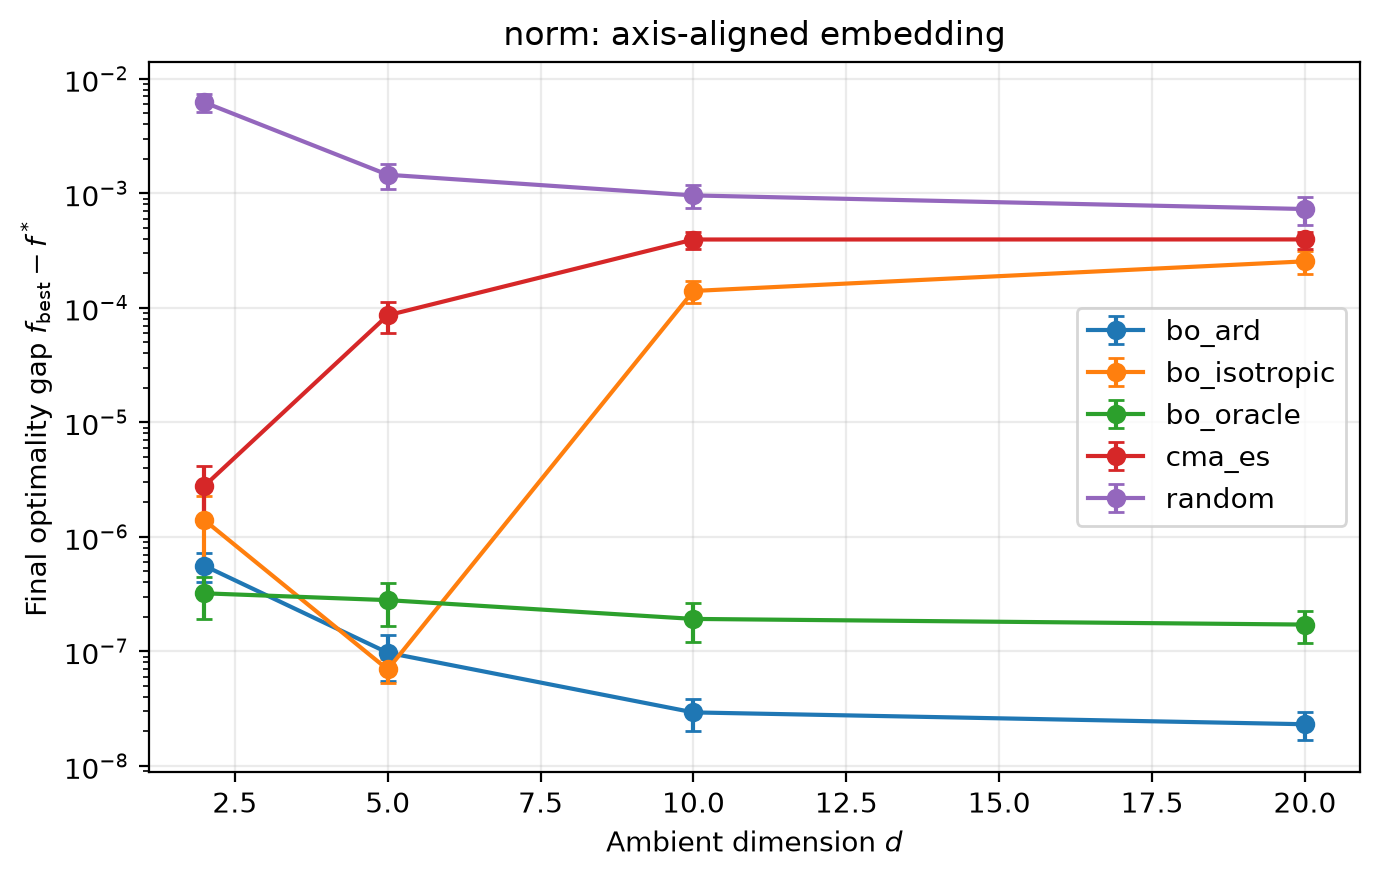
\includegraphics[width=\linewidth]{figures/final_gap_vs_dimension/final_gap_vs_d__norm__aae.png}
        \caption{Norm, aligned}
        \label{fig:dim-norm-aligned}
    \end{subfigure}
    \hfill
    \begin{subfigure}[t]{0.48\textwidth}
        \centering
        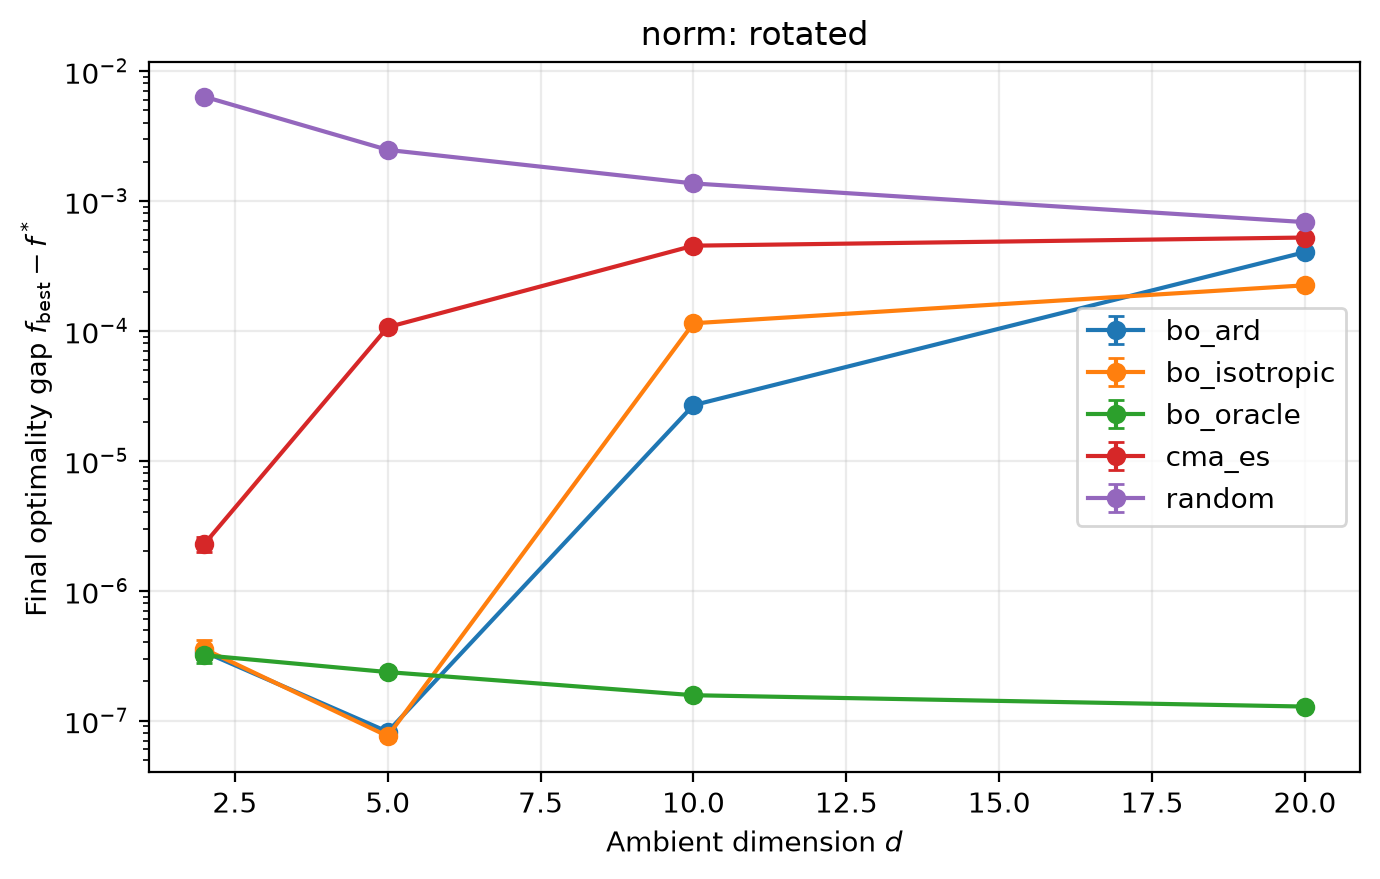
\includegraphics[width=\linewidth]{figures/final_gap_vs_dimension/final_gap_vs_d__norm__rotated.png}
        \caption{Norm, rotated}
        \label{fig:dim-norm-rotated}
    \end{subfigure}

    \vspace{0.4em}

    % Bottom row
    \begin{subfigure}[t]{0.48\textwidth}
        \centering
        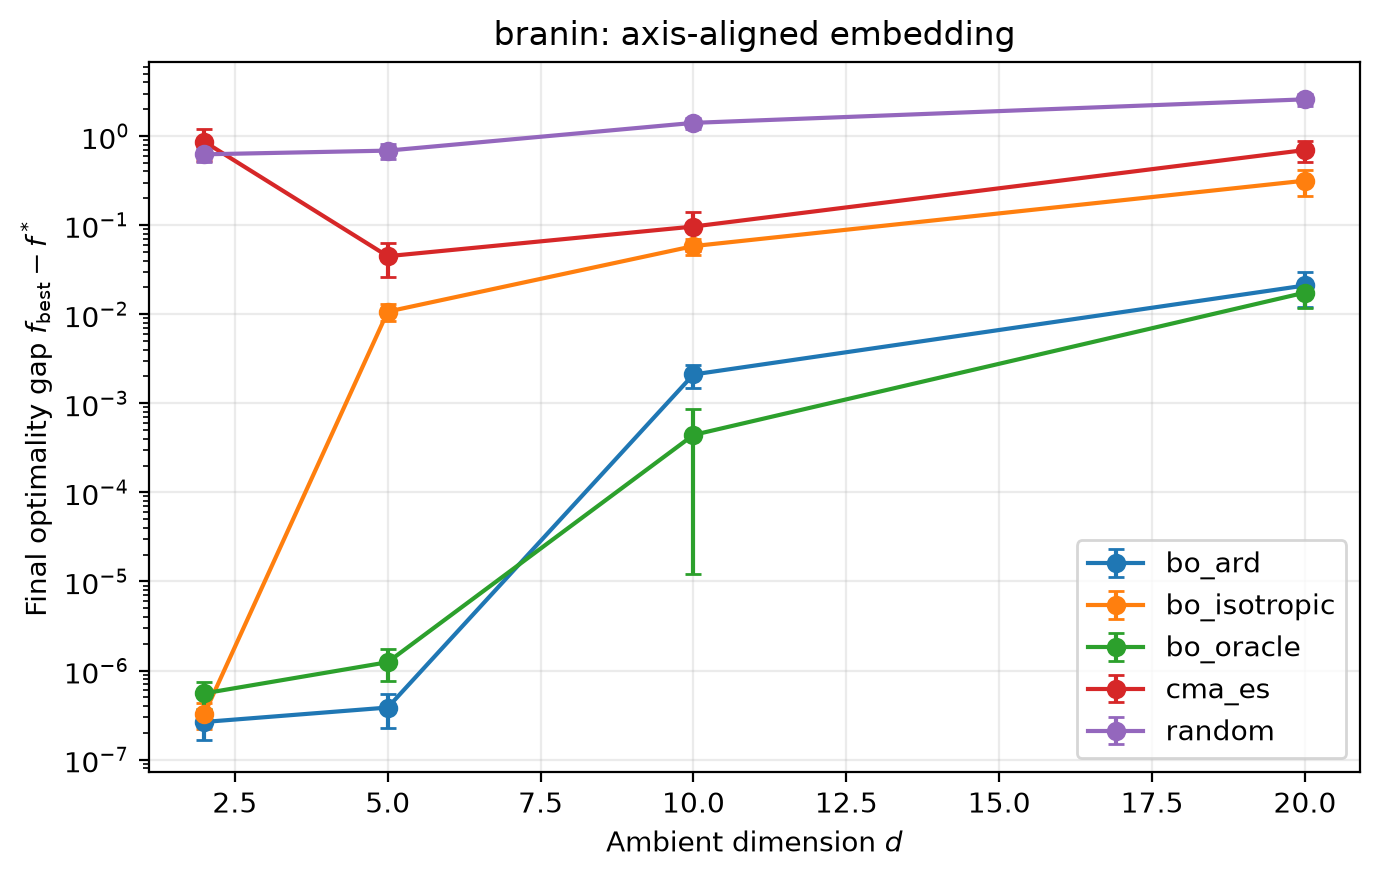
\includegraphics[width=\linewidth]{figures/final_gap_vs_dimension/final_gap_vs_d__branin__aae.png}
        \caption{Branin, aligned}
        \label{fig:dim-branin-aligned}
    \end{subfigure}
    \hfill
    \begin{subfigure}[t]{0.48\textwidth}
        \centering
        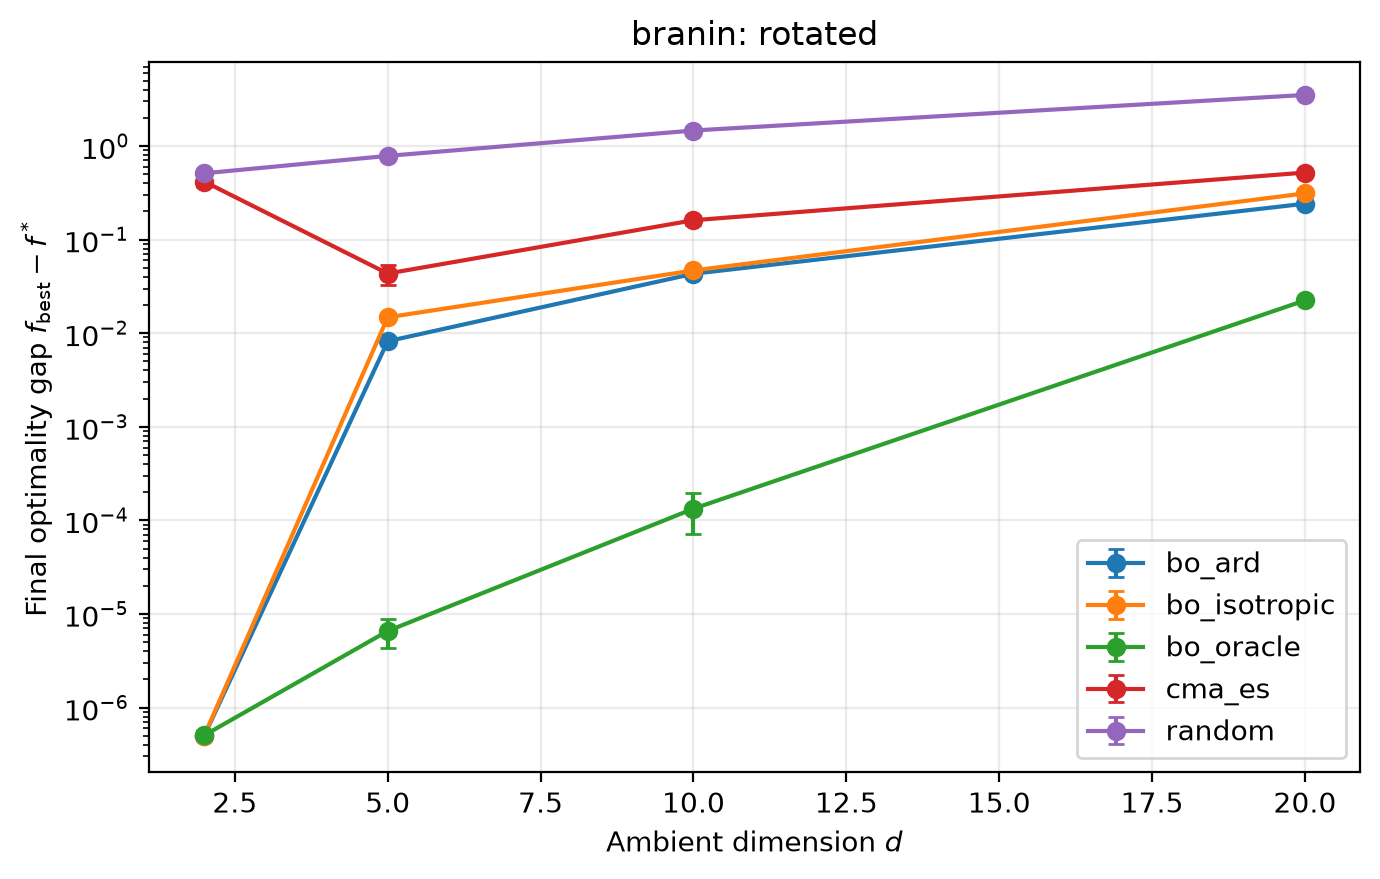
\includegraphics[width=\linewidth]{figures/final_gap_vs_dimension/final_gap_vs_d__branin__rotated.png}
        \caption{Branin, rotated}
        \label{fig:dim-branin-rotated}
    \end{subfigure}

    \caption{Optimality gap as a function of ambient dimension $d$ for the norm and Branin objectives under aligned and rotated active-subspace embeddings.}
    \label{fig:opt-gap-dim}
\end{figure}

Across the four settings---norm and Branin objectives with aligned and rotated embeddings---the optimality gap (see \cref{fig:opt-gap-dim}) generally increases with ambient dimension, partially supporting H1. Several exceptions are observed. Some can be explained by the increasing concentration (\cref{app:projected-distribution}) of projected samples near the origin as $d$ increases, as discussed in \cref{sec:exp-setup}:

\begin{itemize}
    \item \textbf{Random search on the norm objective} (\cref{fig:dim-norm-aligned}, \cref{fig:dim-norm-rotated}) improves with $d$, since the optimum lies at the origin and the projected samples become increasingly concentrated around it.

    \item \textbf{ARD-BO on the aligned norm objective} (\cref{fig:dim-norm-aligned}) similarly improves with $d$. This observation is consistent with the random search phenomenon.

    \item \textbf{Isotropic BO on the norm objective} (\cref{fig:dim-norm-aligned}, \cref{fig:dim-norm-rotated}) initially improves from $d=2$ to $d=5$, before deteriorating at larger $d$. One possible explanation is that the favourable concentration effect initially dominates, but is eventually outweighed by the increasing difficulty of modelling in the ambient space.

    \item \textbf{Oracle BO on Branin} (\cref{fig:dim-branin-aligned}, \cref{fig:dim-branin-rotated}) was expected to remain roughly constant with $d$. However, it deteriorates with $d$, despite operating in the true two-dimensional active space. Unlike the norm objective, the Branin optimum lies away from the origin, so increasingly concentrated initial samples provide less favourable coverage of the optimal region. \textit{Further analysis (\cref{subsec:oracle-dim-problem}) is required to confirm this explanation.}
\end{itemize}

One observation is not immediately explained by this mechanism (\cref{fig:dim-branin-aligned}, \cref{fig:dim-branin-rotated}): CMA-ES on both Branin settings improves from $d=2$ to $d=5$. The cause of this exception remains unclear. 


\subsection{BO outperforms CMA-ES on tight evaluation budget}
Across the tested problems \cref{fig:opt-gap-dim}, nearly all BO variants achieve a lower final optimality gap than CMA-ES. Furthermore, across all dimensions and objective functions, the BO variants consistently outperform CMA-ES throughout the later and substantial majority of the evaluation budget, supporting H2; see \cref{fig:gap-vs-evaluations-eg} for a representative example. This suggests that, in the evaluation-limited regime considered here, the GP surrogate had successfully identified regions with greater potential for improvement.

\begin{figure}[htbp]
    \centering
    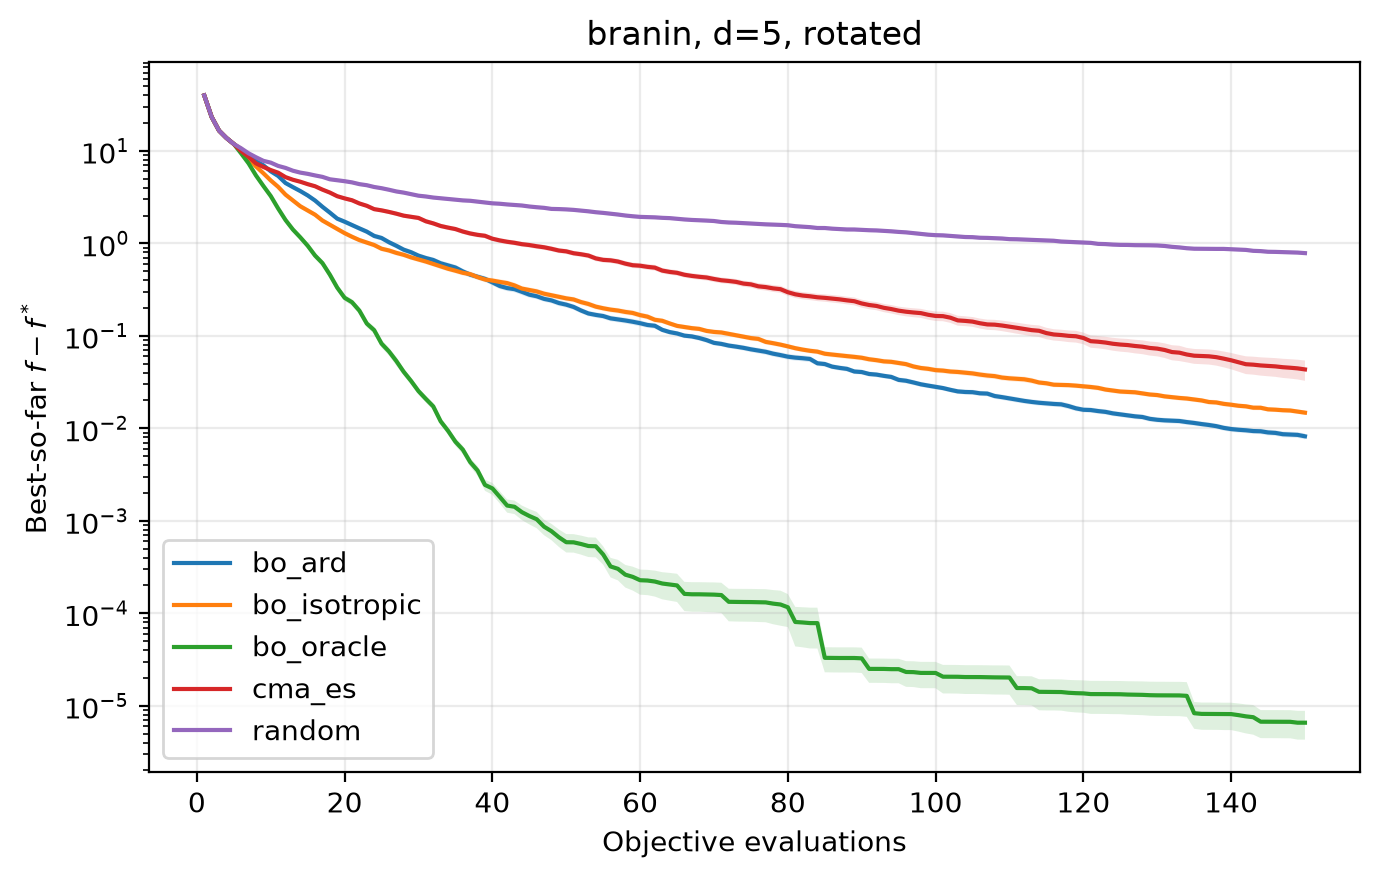
\includegraphics[width=0.75\textwidth]{figures/gap_vs_evaluations/gap_vs_eval__branin__d5__rotated.png}
    \caption{Best-so-far optimality gap $G_t$ against the number of objective evaluations $t$.}
    \label{fig:gap-vs-evaluations-eg}
\end{figure}


\subsection{Sensitivity to alignment}
ARD-BO exhibits the largest deterioration when moving from coordinate-aligned to randomly rotated embeddings for both the norm and Branin objectives, supporting H3. This is consistent with ARD's reliance on coordinate-wise length scales: it can tackle irrelevant coordinates in the aligned case, but struggle to tackle inactive direction that are not axis-aligned.

\begin{figure}[htbp]
    \centering
    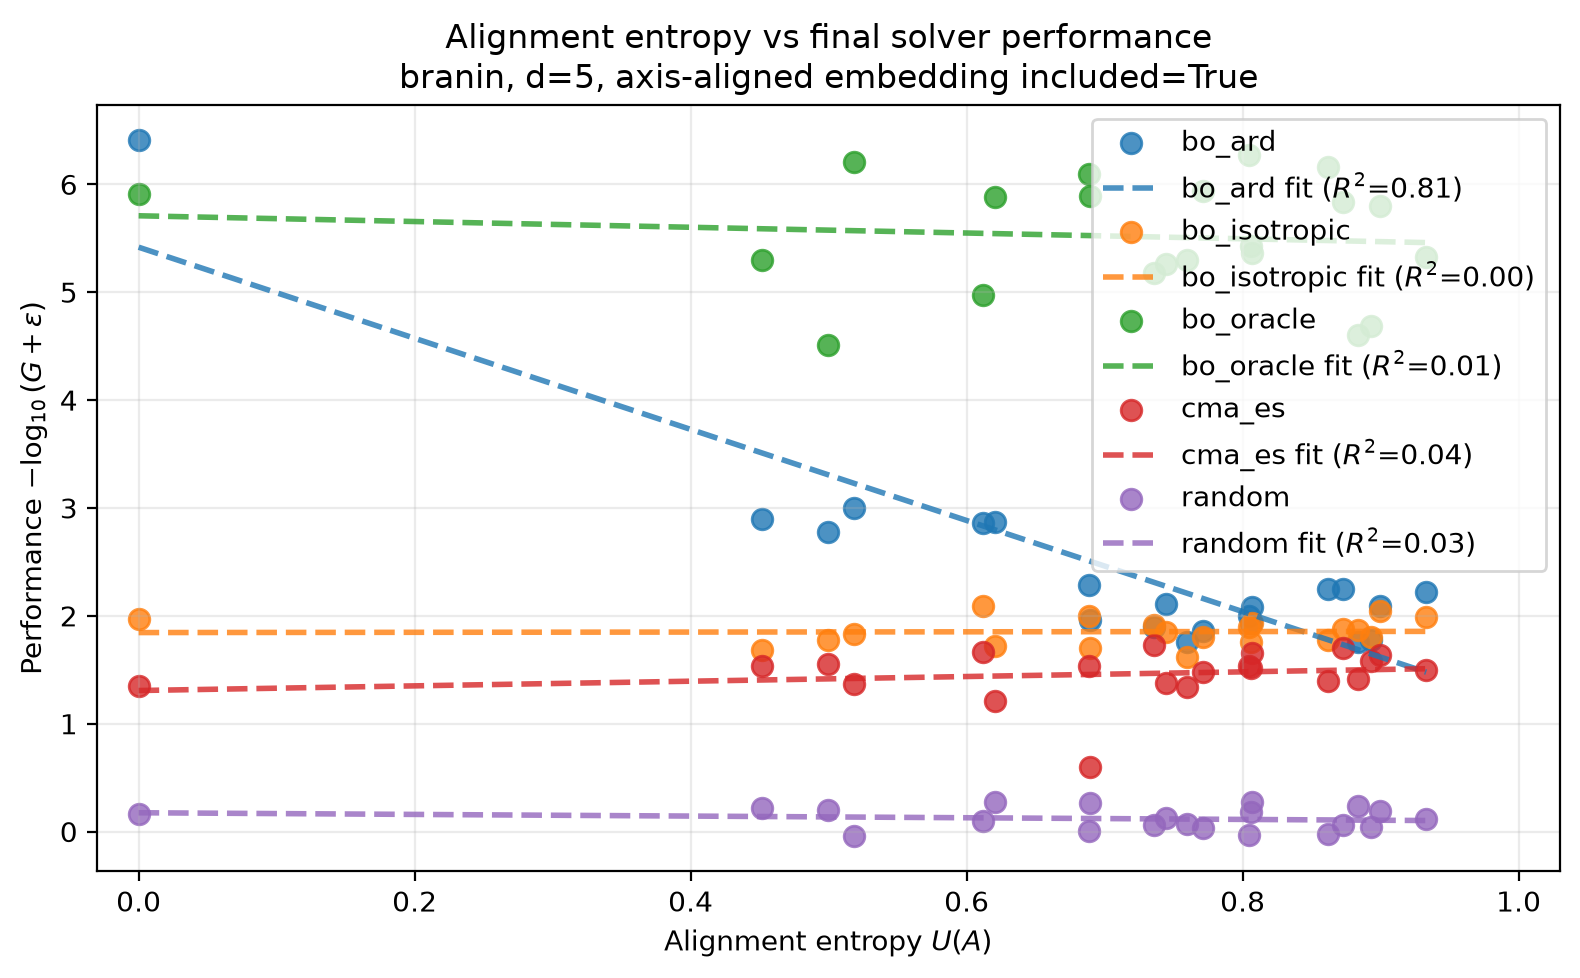
\includegraphics[width=0.75\textwidth]{figures/alignment_entropy/final_performance/alignment_final__branin__d5__with_aae.png}
    \caption{Performance against alignment entropy $U(A)$ for the Branin objective at ambient dimension $d=5$. Lines show the fitted linear regressions for each solver.}
    \label{fig:entropy-performance-d5-branin}
\end{figure}

To assess the rigour of our experiment comparing aligned and non-aligned random matrices $A$, we ask: \textit{how unaligned are the randomly generated active subspaces in practice?} Here, we use the \textbf{alignment entropy} metric to quantify the alignment of those random matrices. \cref{fig:entropy-performance-d5-branin} is a scatter plot (for $d=5, g=\mathrm{Branin}$) of $\mathrm{Perf}$ against alignment entropy. The points with alignment entropy $0$ corresponds to $A_\mathrm{inc}$, the aligned matrices, while we observe that the random non-aligned matrices have alignment entropy spread between $0.4$ and $1.0$, suggesting that the gap is sufficient to test the difference in performance.

Additionally, we observe that The fitted ARD-BO regression has a visibly more negative slope than those of the other solvers. This is generally true (\cref{fig:entropy-performance-all}) for all values of $d$ and objectives $g$.

\subsection{Oracle having the best performance}
In \cref{fig:opt-gap-dim}, we observe that oracle BO performs better than all other models for non-aligned embeddings. However, the performance of oracle BO is roughly the same as ARD-BO for the axis-aligned case when $g = \mathrm{Branin}$. When $g=\mathrm{norm}$, ARD-BO performs unexpectedly better than oracle BO for $d \geq 5$, which is surprising, given that oracle BO knows the embedded subspace. 

One possible explanation is that ARD-BO has two active length scales as compared to one for oracle, allowing for greater adaptation to the optimisation landscape. However, this explanation is not convincing as the $\mathrm{norm}$ objective is symmetric on the two axes. \textit{Further analysis (\cref{subsec:ard-outperform-oracle-problem}) is required.}

\section{Further analysis}
\subsection{Oracle BO performs worse as $d$ increases}
\label{subsec:oracle-dim-problem}
Oracle BO was expected to be largely insensitive to ambient dimension because its GP operates directly on the true \(k=2\) active coordinates. However, for the Branin objective, its performance deteriorates as \(d\) increases. Inspection (\cref{fig:oracle-branin-trajectory}) of the evaluation trajectories shows that evaluation points increasingly cluster near the origin of the active space, with this concentration becoming stronger at larger \(d\). Since the Branin optimum lies away from the origin, this reduces the ability of Oracle BO to explore the optimal region.

A likely source of this behaviour is the acquisition optimisation procedure where candidates sampled uniformly from the ambient unit ball \(B^d\). Their projections \(A^\top x\) become increasingly concentrated near the origin as \(d\) increases. Consequently, the candidate used to initialise local acquisition optimisation is drawn from an increasingly concentrated distribution on the embedded subspace. Thus, while the Oracle surrogate itself is independent of ambient dimension, its acquisition-optimisation procedure is not. Further implementation details are provided in \cref{app:oracle-implementation}.
 

\subsection{ARD BO outperforms oracle BO}
\label{subsec:ard-outperform-oracle-problem}
ARD-BO unexpectedly outperforms Oracle BO on the axis-aligned norm objective for \(d>2\) (\cref{fig:ard-oracle-improvement}). The fitted ARD length scales (\cref{fig:ard-oracle-length-scales}) show that inactive coordinates receive very large length scales, confirming that ARD successfully identifies and suppresses them. However, this does not itself explain the advantage over Oracle, which already knows the active subspace.

At \(d=2\) (\cref{fig:active-ls-d2}), ARD and Oracle learn similar length scales and achieve similar improvements. For \(d>2\) (\cref{fig:active-ls-d5}, \cref{fig:active-ls-d10}, \cref{fig:active-ls-d20}), ARD learns substantially smaller active length scales and achieves greater improvement from initialization. This suggests that ARD's advantage is associated with a more local surrogate in the active space, although why ARD learns these smaller length scales, and whether they directly cause the performance improvement, remains unclear.


% ============================================================
\section{Limitations}

\paragraph{Small problem set} Due to computational and time constraints, our experiments are restricted to effective dimension \(k=2\), $g = \mathrm{norm}, \mathrm{Branin}$, with \(n_{\mathrm{init}}=20\) initialisation sets and \(n_{\mathrm{rot}}=20\) random embeddings. Hence, the results may not fully generalise to higher effective dimensions, real black-box problems and capture the full variability across problem instances respectively.

\paragraph{Dependence on ambient domain} Our results depend on the choice of ambient domain. The rotationally invariant unit ball \(B^d\) enables fair comparison across subspace orientations, but its projected distribution becomes increasingly concentrated near the origin as \(d\) increases, affecting optimisation performance. A hypercube may better represent real-world problems where individual variables are bounded by intervals, but it sacrifices rotational invariance, such that the projected distribution depends on the orientation of the active subspace. Therefore, some of our conclusions that are specific to the chosen domain, may not reflect real-world problems. 

\section{Conclusion}

Our experiments broadly support the four proposed hypotheses. Performance generally deteriorates as ambient dimension increases, although this effect depends on the objective and domain geometry. Under the tested evaluation budget, BO is more evaluation-efficient than CMA-ES. ARD-BO benefits strongly from coordinate-aligned low-dimensional structure and deteriorates under rotation, while Oracle BO generally performs best for non-aligned embeddings, demonstrating the value of knowing the active subspace.

Several exceptions to these hypotheses motivated further investigation. Practical implementation choices can reintroduce ambient-dimensional effects even when the Oracle surrogate itself operates entirely in the effective space. Furthermore, ARD-BO can successfully recover axis-aligned low-dimensional structure while learning a surrogate geometry distinct from Oracle BO. These findings highlight that the performance of black-box optimisers depends not only on ambient and effective dimension, but also on problem geometry and practical implementation choices.

 

\newpage
\appendix

\section*{Appendix}

\section{Properties of the Projected Distribution}
\label{app:projected-distribution}


Let $X\sim\operatorname{Unif}(B^d(1))$ be uniformly distributed
over the $d$-dimensional unit ball
$B^d(1)=\{x\in\mathbb R^d:\|x\|_2\leq1\}$.
This means that for any Lebesgue-measurable set
$S\subseteq B^d(1)$,
\[
\mathbb P(X\in S)
=\frac{\lambda_d(S)}{\lambda_d(B^d(1))},
\]
where $\lambda_d$ denotes the $d$-dimensional Lebesgue measure.

Let $Z=A^\top X\in\mathbb R^k$ denote the projection of $X$
onto a $k$-dimensional subspace, where $A^\top A=I_k$.
The squared norm of the projected vector follows a Beta distribution:
\[
\|Z\|_2^2\sim
\operatorname{Beta}\left(\frac{k}{2},\frac{d-k}{2}+1\right).
\]
Consequently,
\[
\mathbb E[\|Z\|_2^2]=\frac{k}{d+2}.
\]

Thus, for fixed $k$, the expected squared distance of the
projected points from the origin decreases as the ambient
dimension $d$ increases, indicating increasing concentration
near the origin.

% Supporting derivation/proof:
% - rotational invariance
% - concentration near the origin as d increases

\section{Alignment Entropy Metric}
\label{app:alignment-entropy}

Let $P=AA^\top$ be the orthogonal projection matrix onto the active subspace. We can study the diagonal of $P$, to determine how ``non-aligned" a subspace is. 

Looking at its properties, firstly, the $i$-th diagonal element of $P=AA^\top$ is given by $P_{ii}=\sum_{j=1}^{k}A_{ij}^2=\|A^\top e_i\|_2^2$. Since $P_{ii}\geq 0$ and $A$ orthonormal, we have $P_{ii}\in[0,1]$ for all $i=1,\ldots,d$. Secondly, we observe that if the subspace is axis-aligned, $\mathrm{diag}(P)$ will contain $k$ $1$'s with the remaining $d-k$ entries being $0$. Since $\operatorname{tr}(P)=k$, we expect that $\mathrm{diag}(P)$ being uniformly distributed and having $\frac kd$ as all its entries will indicate the the subspace is extremely ``unaligned''. 

Define
\[
    p_i=\frac{P_{ii}}{k},
    \qquad
    H(A)=-\sum_{i=1}^{d}p_i\log p_i,
\]
where $p_1,\ldots,p_d$ form a probability distribution (by the first observation) and $H(A)$ measures how evenly the active subspace is distributed across the ambient coordinates (by the second observation). Since the lower bound is $\log k$, we define the normalized alignment entropy as
\begin{equation}
    U(A)
    =
    \frac{H(A)-\log k}{\log d-\log k}.
\end{equation}

Thus, $U(A)=1$ if and only if the diagonal entries of $P$ are uniform, with $P_{ii}=k/d$ for all $i$. Additionally, with the condition that $P_{ii} \leq 1$, one can show that $U(A)=0$ if and only if the diagonal of $P$ contains exactly $k$ entries equal to $1$, with all remaining entries equal to $0$.


\section{Implementation of Oracle BO}
\label{app:oracle-implementation}

Oracle BO assumes knowledge of the true active-subspace matrix
$A\in\mathbb{R}^{d\times 2}$. The intended Oracle covariance between two
ambient points $x,x'\in\mathbb{R}^d$ is
\[
k_A(x,x')
=
\sigma_f^2
\exp\left(
-\frac{\|A^\top(x-x')\|_2^2}{2\ell^2}
\right).
\]

Rather than implementing this projected kernel explicitly, we exploit its
equivalence to a standard RBF kernel in the effective space. For every
evaluated point $x_i$, we compute
$
z_i=A^\top x_i\in\mathbb{R}^2.
$
The Oracle GP is then fitted to the transformed observations
$
\mathcal D_n^{\mathrm{Oracle}}
=
\{(z_i,y_i)\}_{i=1}^n
$
using the two-dimensional isotropic RBF kernel
\[
k(z,z')
=
\sigma_f^2
\exp\left(
-\frac{\|z-z'\|_2^2}{2\ell^2}
\right).
\]
Since
$
z-z'=A^\top(x-x'),
$
this gives exactly the same covariance as applying $k_A(x,x')$ directly
to the ambient points. The fitted two-dimensional GP therefore defines
an Expected Improvement acquisition function $\operatorname{EI}(z)$.

The next evaluation point must lie in the ambient
search domain $B^d$. Thus, we define the acquisition function as
\[
\alpha(x)
=
\operatorname{EI}(A^\top x),
\]
and seek
\[
x_{\mathrm{next}}
=
\arg\max_{x\in B^d}
\operatorname{EI}(A^\top x).
\]

Acquisition optimization (this is performed similarly for other BO variants) is performed using a random-search
initialization followed by local constrained optimization. \textit{At each BO
iteration, \newline \texttt{n\_candidates=1500} candidate points are sampled
uniformly from $B^d$.} We proceed to rank them accordingly to their $\alpha$ values, and the best
\texttt{n\_acq\_starts=1} candidate(s) is used as the starting point for
local optimization via Sequential Least Squares Programming (SLSQP).  The
resulting feasible maximizer is selected as $x_{\mathrm{next}}$. If the
SLSQP optimization is unsuccessful, the best point among the original
\texttt{n\_candidates}$=1500$ random candidates is used instead.

Finally, the embedded objective is evaluated at the selected point, and 
$
\left(z_\mathrm{next}=A^\top x_{\mathrm{next}},f(x_\mathrm{next})\right)
$
is then added to the Oracle GP training data. The GP is refitted and the
procedure is repeated until the evaluation budget is exhausted.



\FloatBarrier
\section{Additional Plots}

\begin{figure}[htbp]
    \centering

    % Row 1: Norm
    \begin{subfigure}[t]{0.32\textwidth}
        \centering
        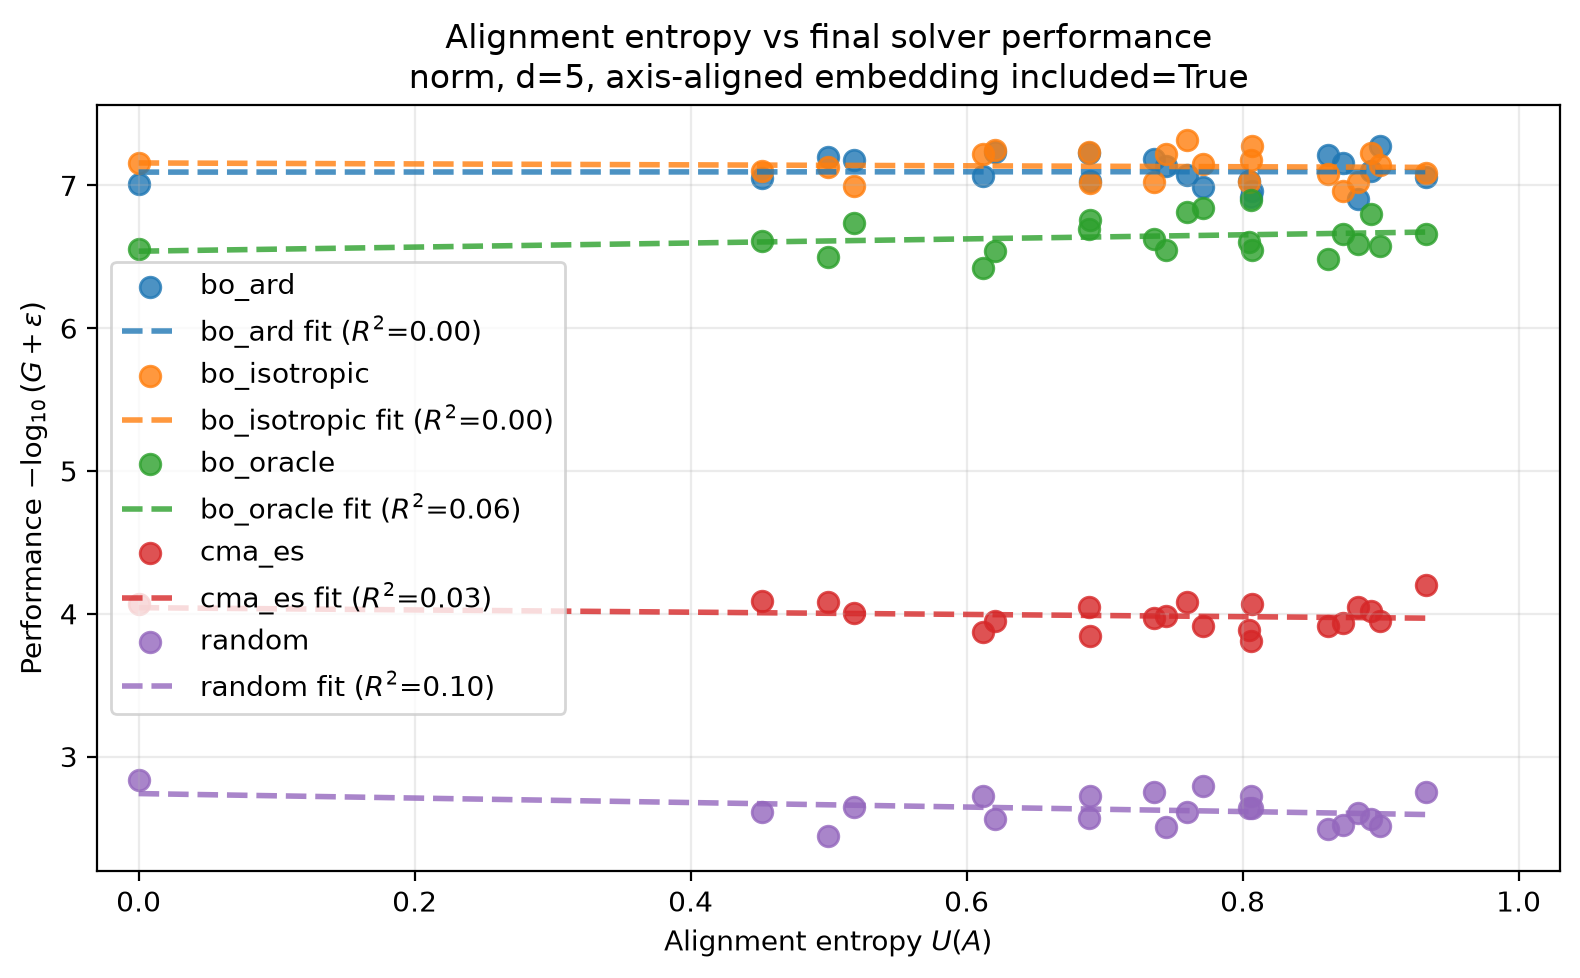
\includegraphics[width=\linewidth]{figures/alignment_entropy/final_performance/alignment_final__norm__d5__with_aae.png}
        \caption{Norm, $d=5$}
        \label{fig:entropy-norm-d5}
    \end{subfigure}
    \hfill
    \begin{subfigure}[t]{0.32\textwidth}
        \centering
        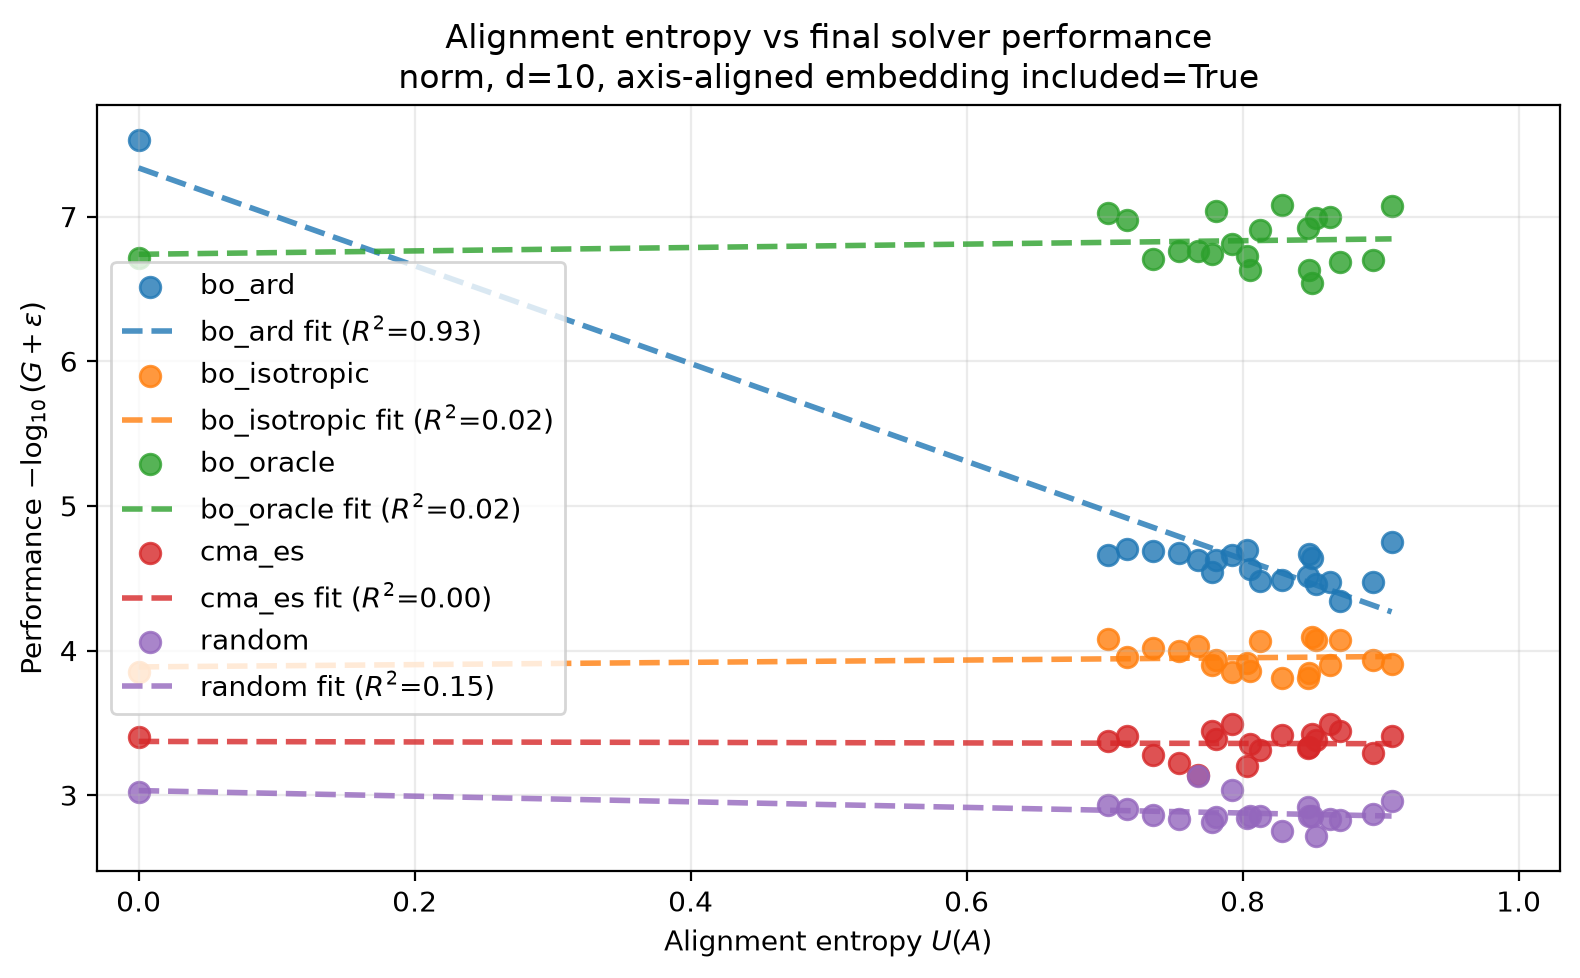
\includegraphics[width=\linewidth]{figures/alignment_entropy/final_performance/alignment_final__norm__d10__with_aae.png}
        \caption{Norm, $d=10$}
        \label{fig:entropy-norm-d10}
    \end{subfigure}
    \hfill
    \begin{subfigure}[t]{0.32\textwidth}
        \centering
        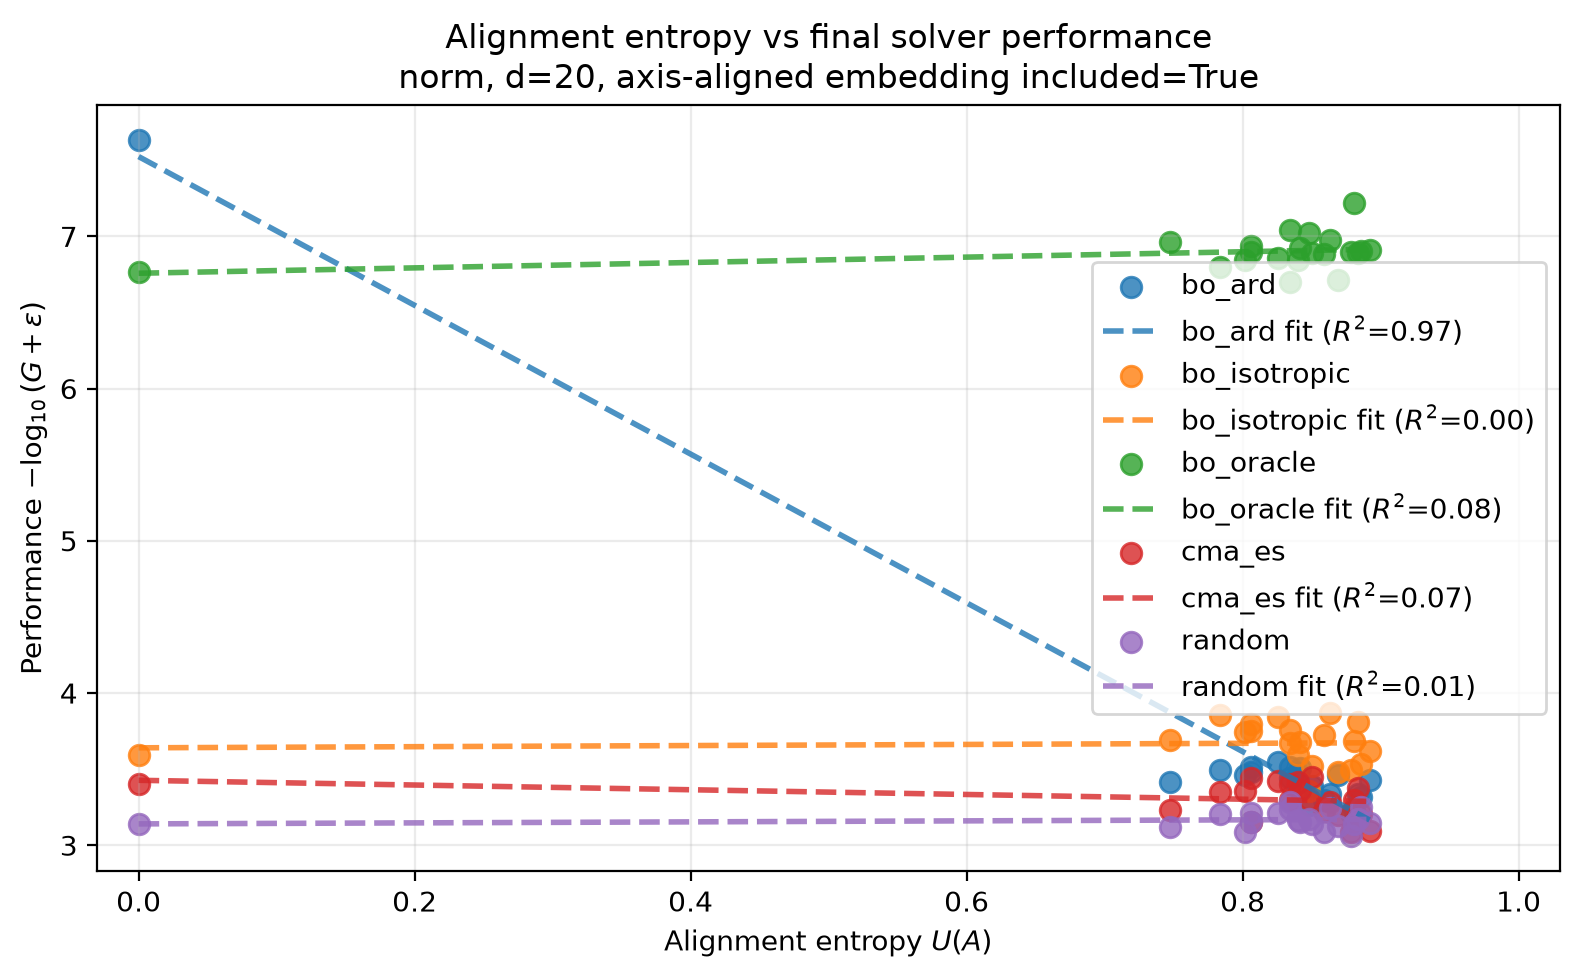
\includegraphics[width=\linewidth]{figures/alignment_entropy/final_performance/alignment_final__norm__d20__with_aae.png}
        \caption{Norm, $d=20$}
        \label{fig:entropy-norm-d20}
    \end{subfigure}

    \vspace{0.5em}

    % Row 2: Branin
    \begin{subfigure}[t]{0.32\textwidth}
        \centering
        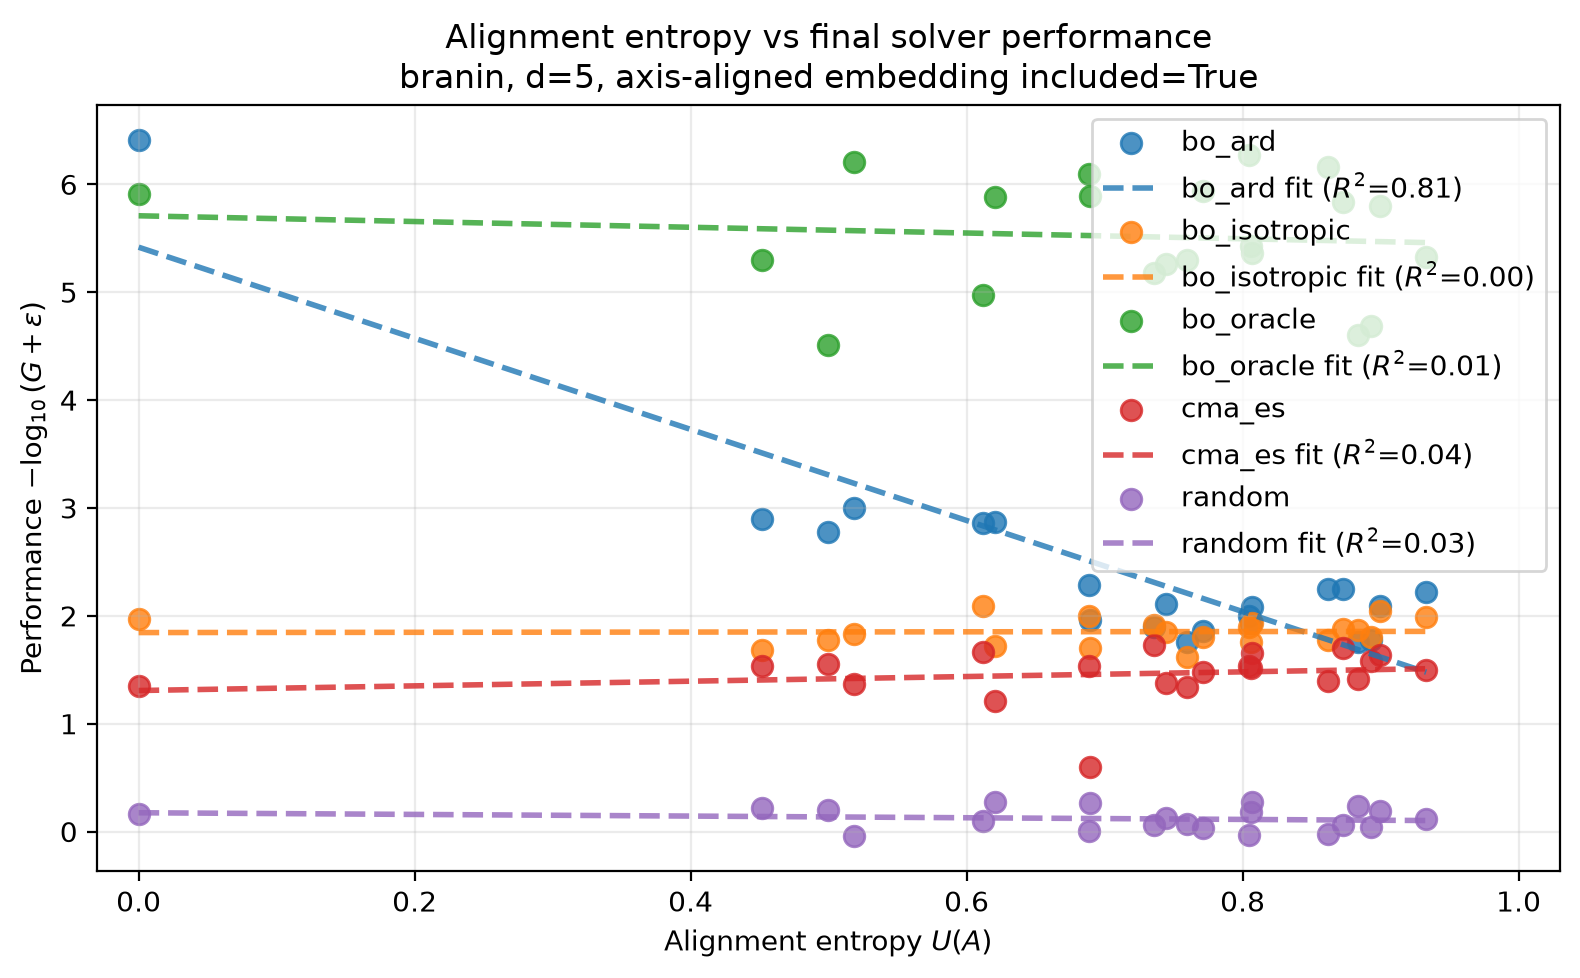
\includegraphics[width=\linewidth]{figures/alignment_entropy/final_performance/alignment_final__branin__d5__with_aae.png}
        \caption{Branin, $d=5$}
        \label{fig:entropy-branin-d5}
    \end{subfigure}
    \hfill
    \begin{subfigure}[t]{0.32\textwidth}
        \centering
        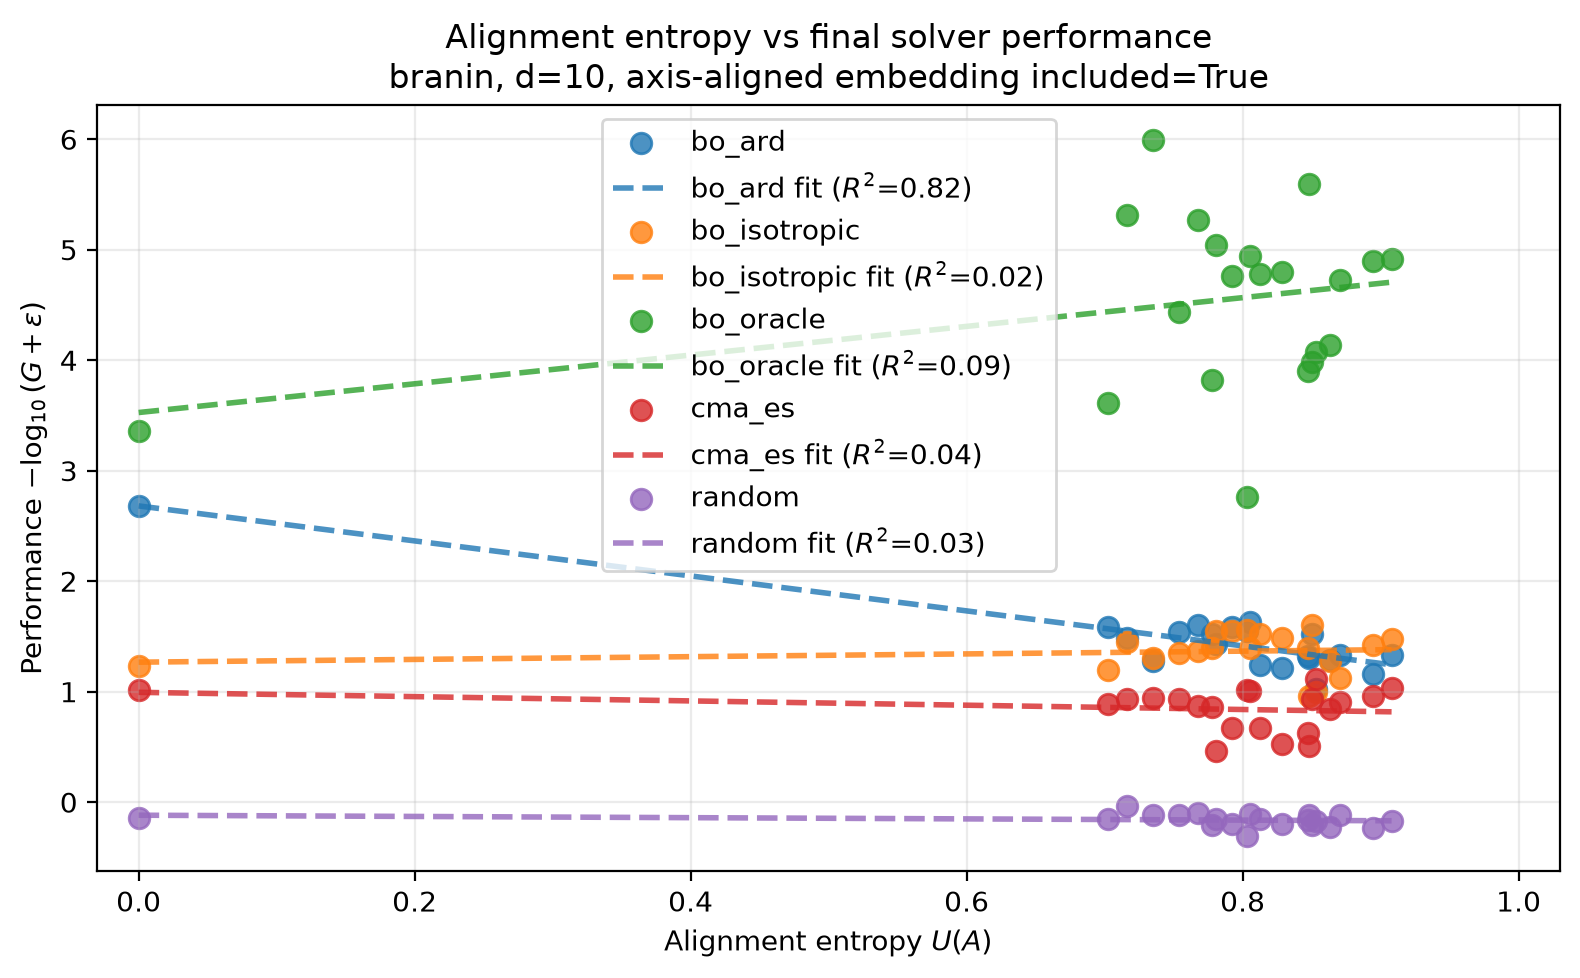
\includegraphics[width=\linewidth]{figures/alignment_entropy/final_performance/alignment_final__branin__d10__with_aae.png}
        \caption{Branin, $d=10$}
        \label{fig:entropy-branin-d10}
    \end{subfigure}
    \hfill
    \begin{subfigure}[t]{0.32\textwidth}
        \centering
        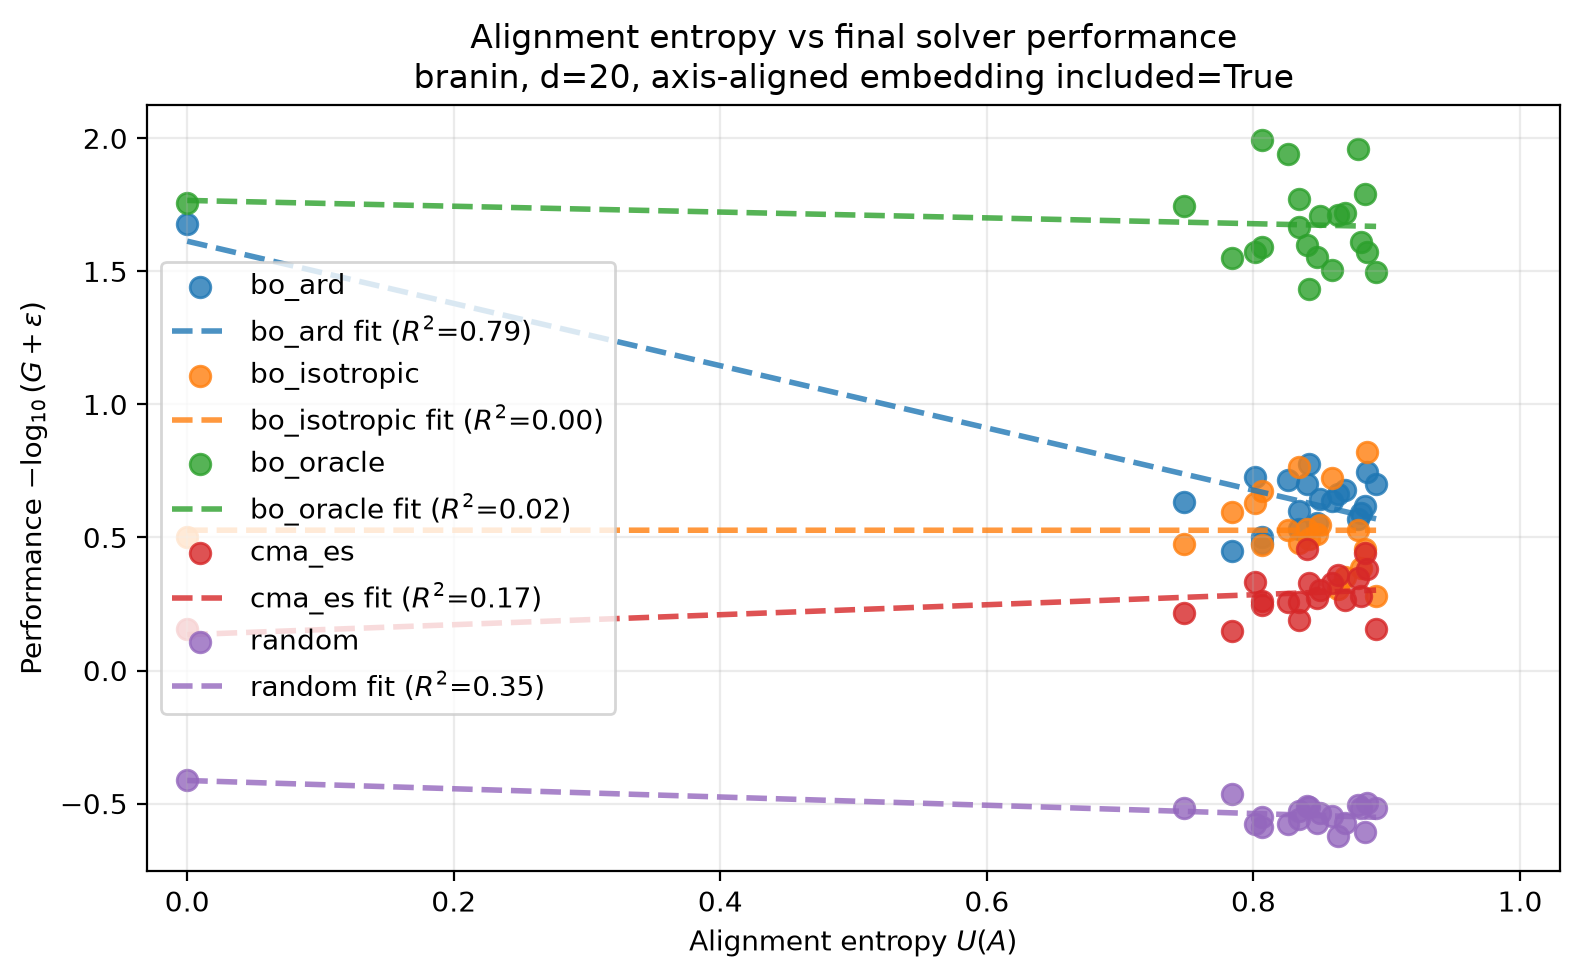
\includegraphics[width=\linewidth]{figures/alignment_entropy/final_performance/alignment_final__branin__d20__with_aae.png}
        \caption{Branin, $d=20$}
        \label{fig:entropy-branin-d20}
    \end{subfigure}

    \caption{Performance against alignment entropy $U(A)$ for the norm and Branin objectives at ambient dimensions $d\in\{5,10,20\}$. Lines indicate the fitted linear regressions for each solver.}
    \label{fig:entropy-performance-all}
\end{figure}
\begin{figure}[htbp]
    \centering
    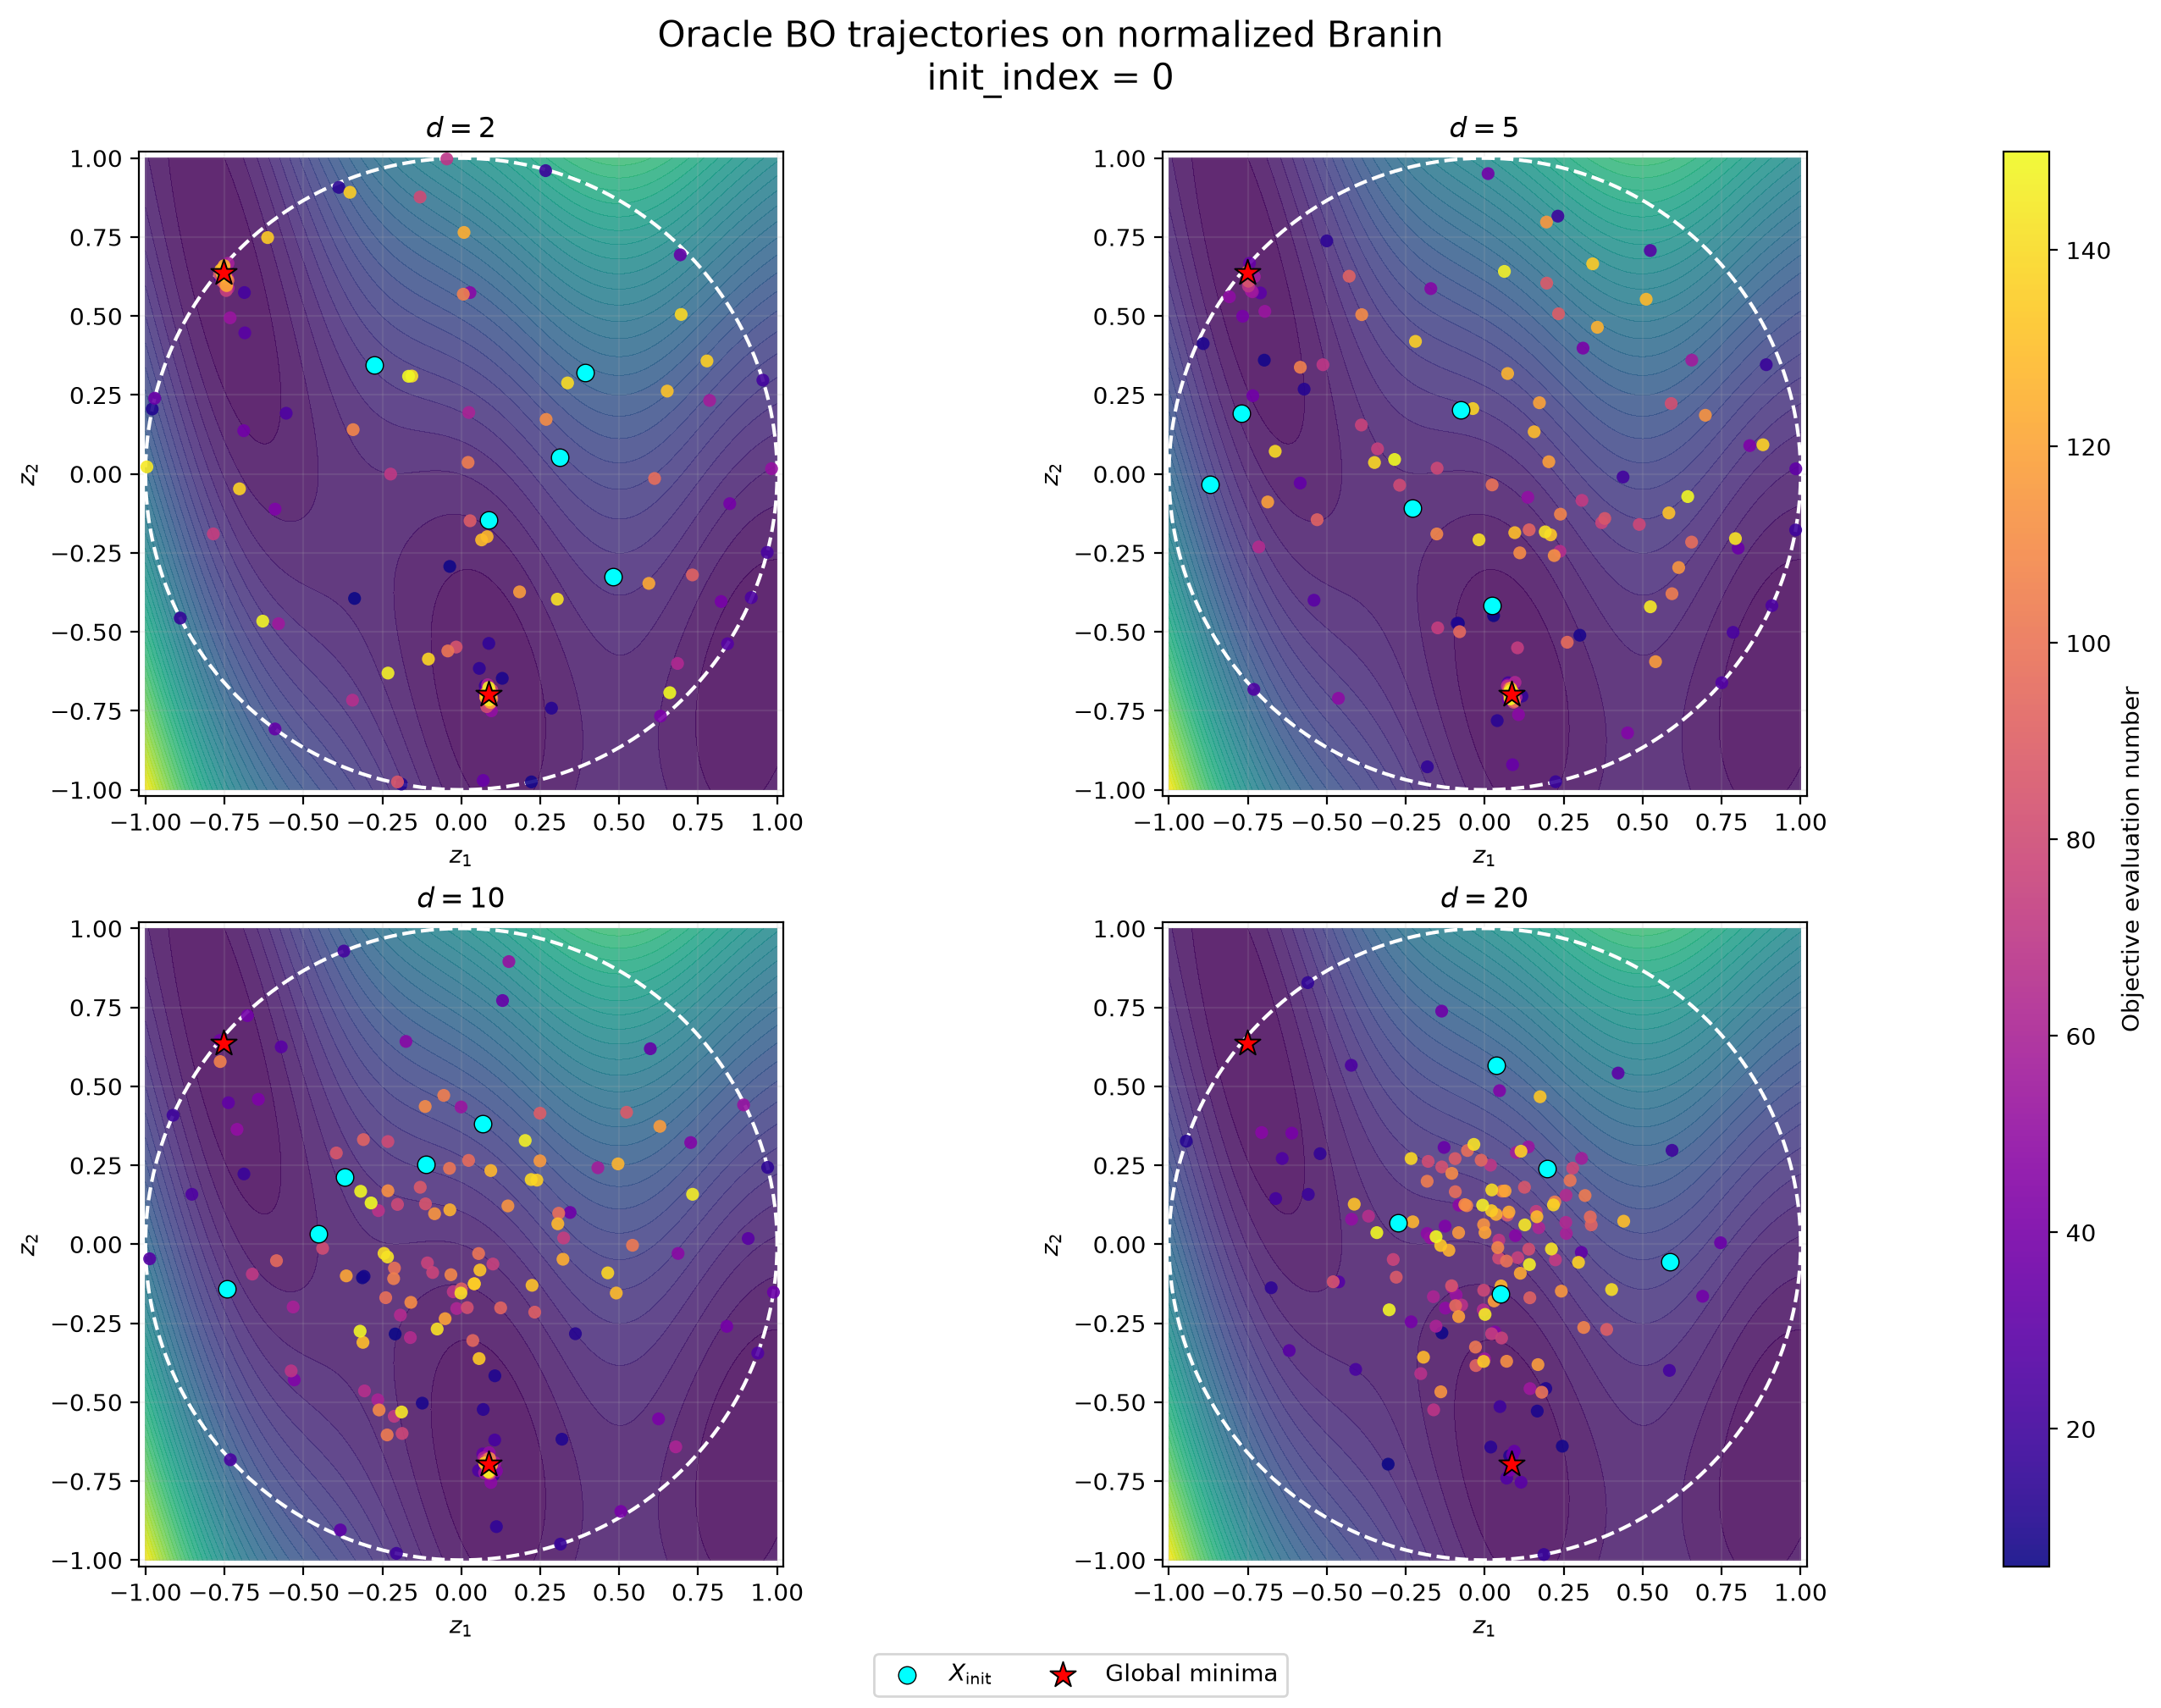
\includegraphics[width=0.8\textwidth]
    {figures/diagnostics_oracle_dim/oracle_branin_trajectory__init0.png}
    \caption{Oracle BO evaluation trajectories for the Branin objective across ambient dimensions. The projected evaluations become increasingly concentrated near the origin as $d$ increases.}
    \label{fig:oracle-branin-trajectory}
\end{figure}

% ARD vs Oracle improvement
\begin{figure}[htbp]
    \centering
    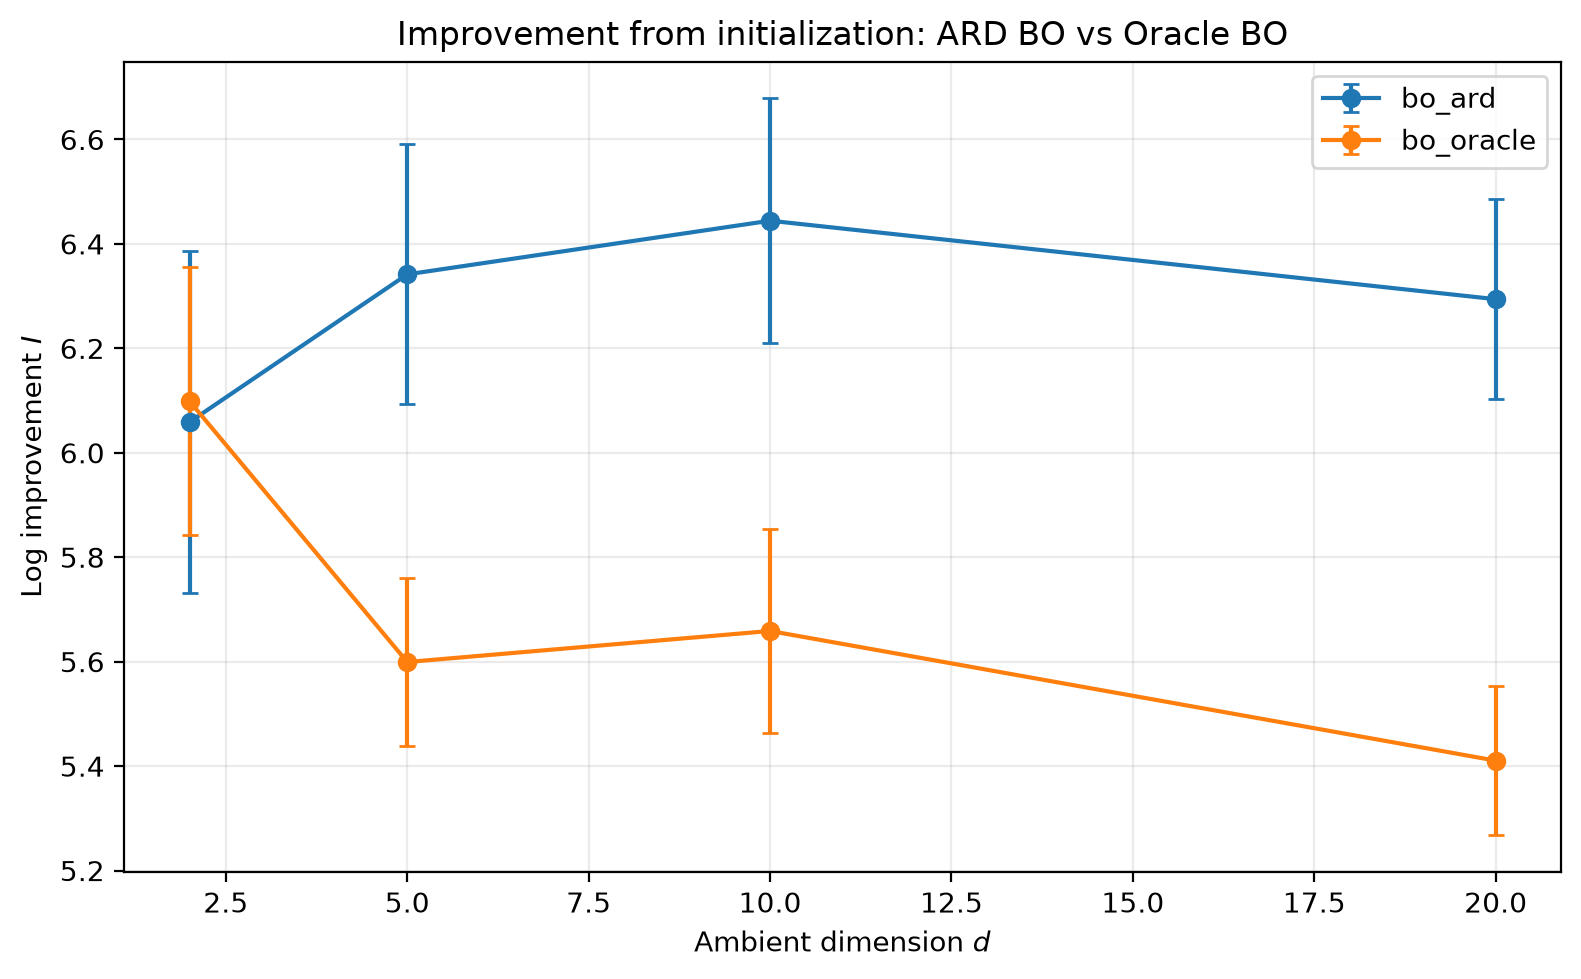
\includegraphics[width=0.75\textwidth]
    {figures/diagnostics_ard_oracle/log_improvement__ard_vs_oracle.png}
    \caption{Improvement from initialization for ARD-BO and Oracle BO on the axis-aligned norm objective.}
    \label{fig:ard-oracle-improvement}
\end{figure}


% Active length-scale trajectories
\begin{figure}[htbp]
    \centering

    \begin{subfigure}[t]{0.48\textwidth}
        \centering
        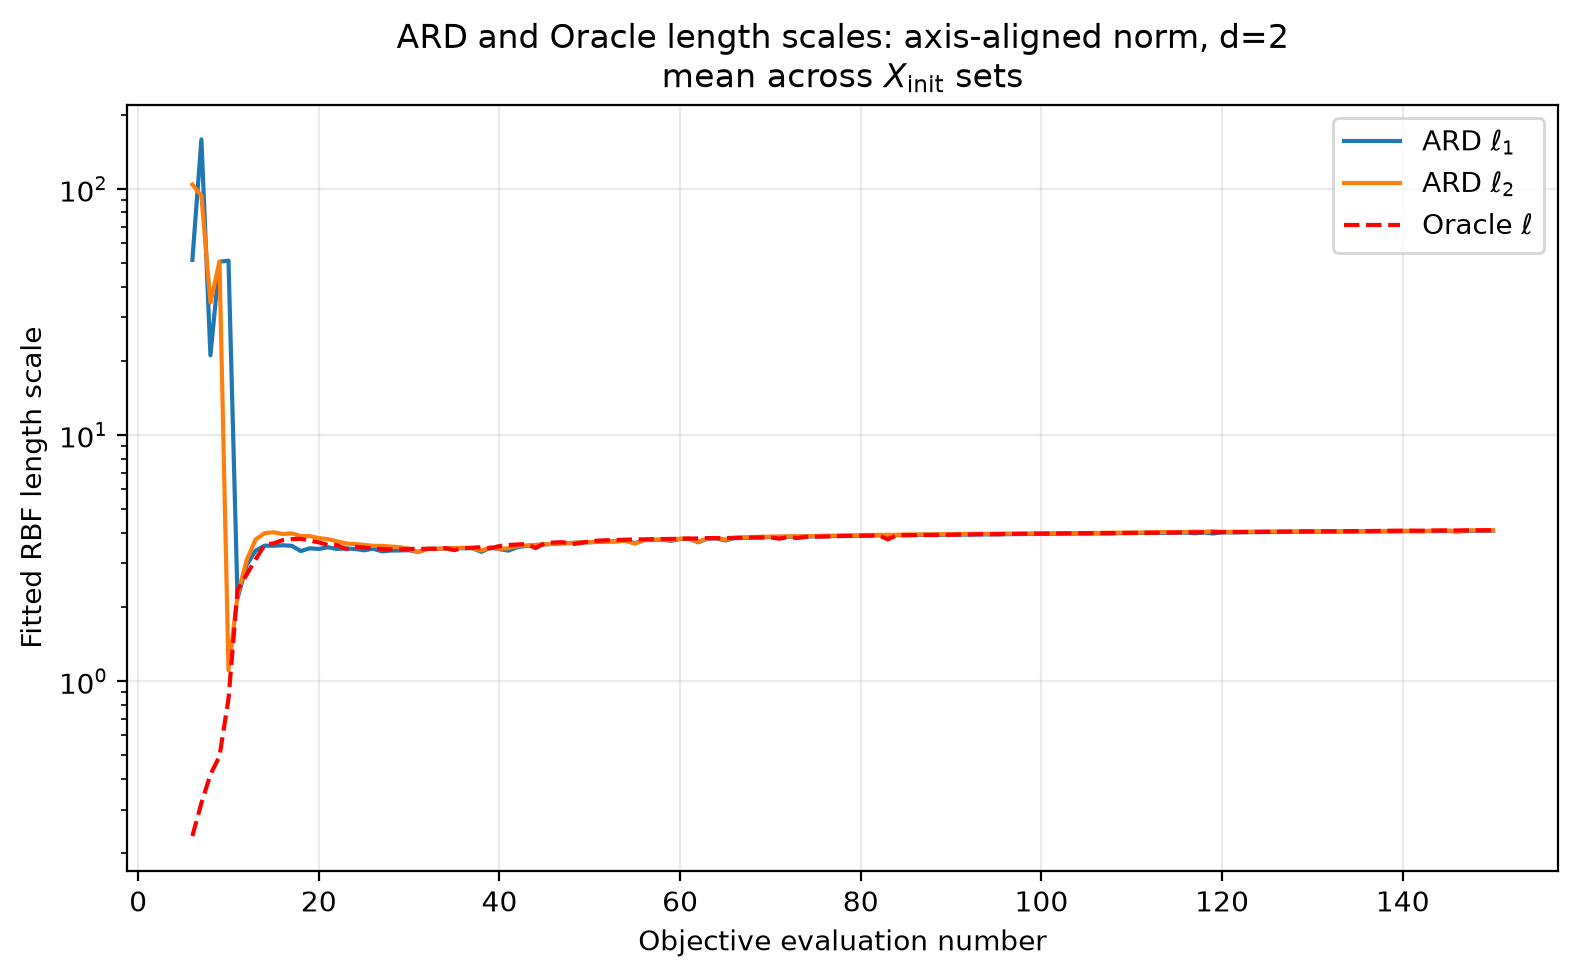
\includegraphics[width=\linewidth]
        {figures/diagnostics_ard_oracle/length_scales__d2.png}
        \caption{$d=2$}
        \label{fig:active-ls-d2}
    \end{subfigure}
    \hfill
    \begin{subfigure}[t]{0.48\textwidth}
        \centering
        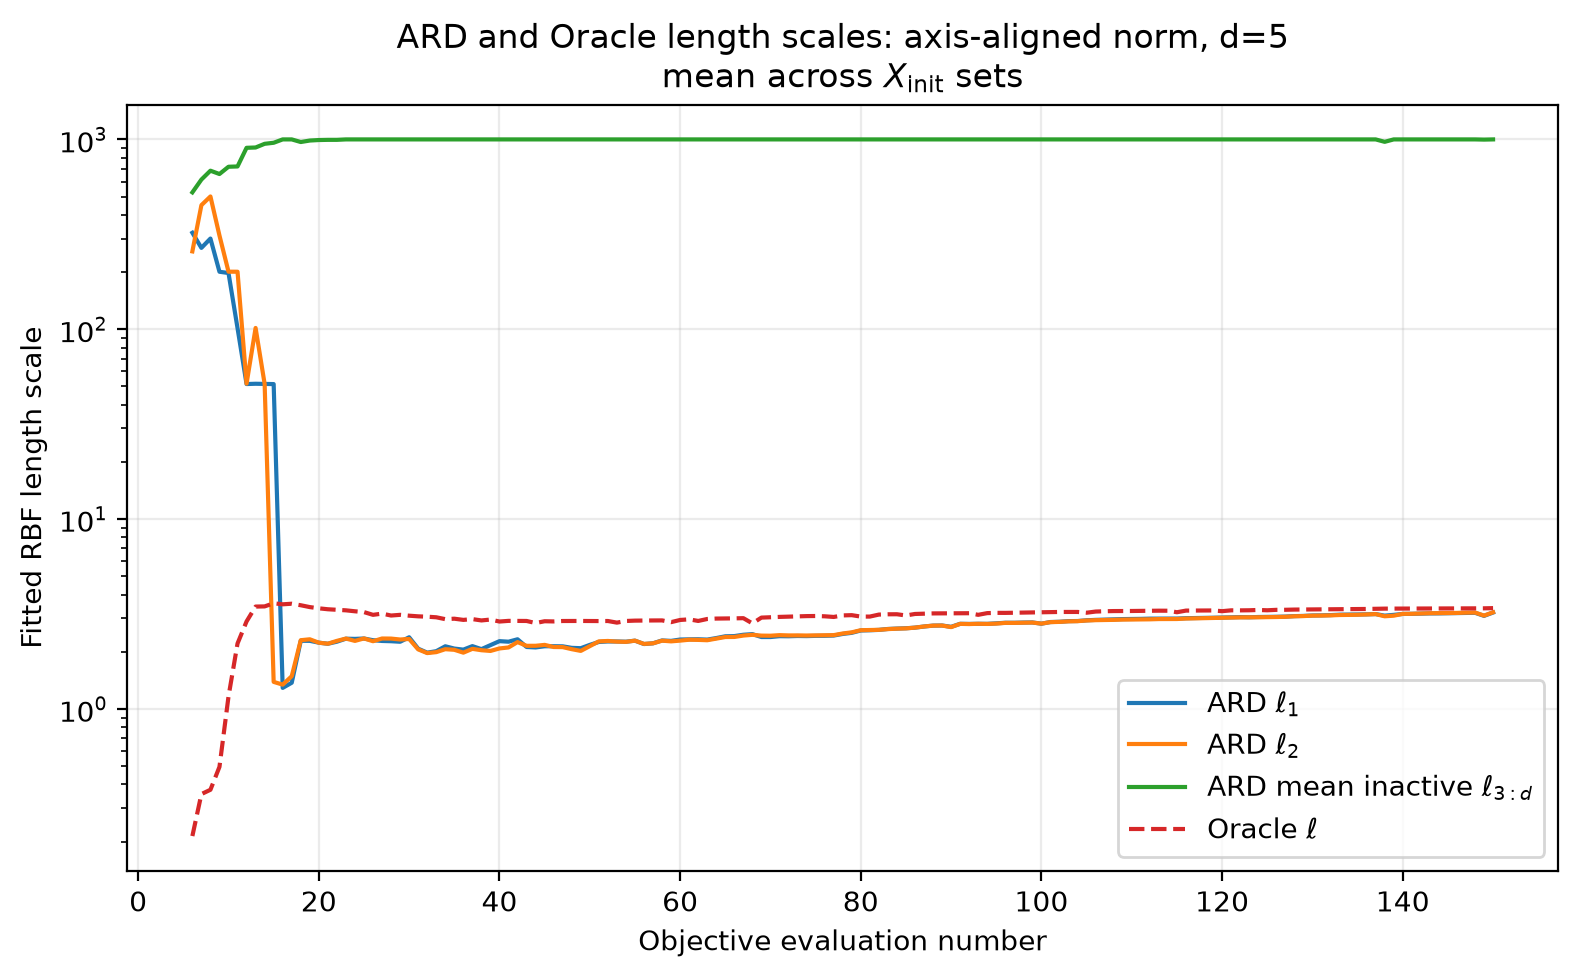
\includegraphics[width=\linewidth]
        {figures/diagnostics_ard_oracle/length_scales__d5.png}
        \caption{$d=5$}
        \label{fig:active-ls-d5}
    \end{subfigure}

    \vspace{0.4em}

    \begin{subfigure}[t]{0.48\textwidth}
        \centering
        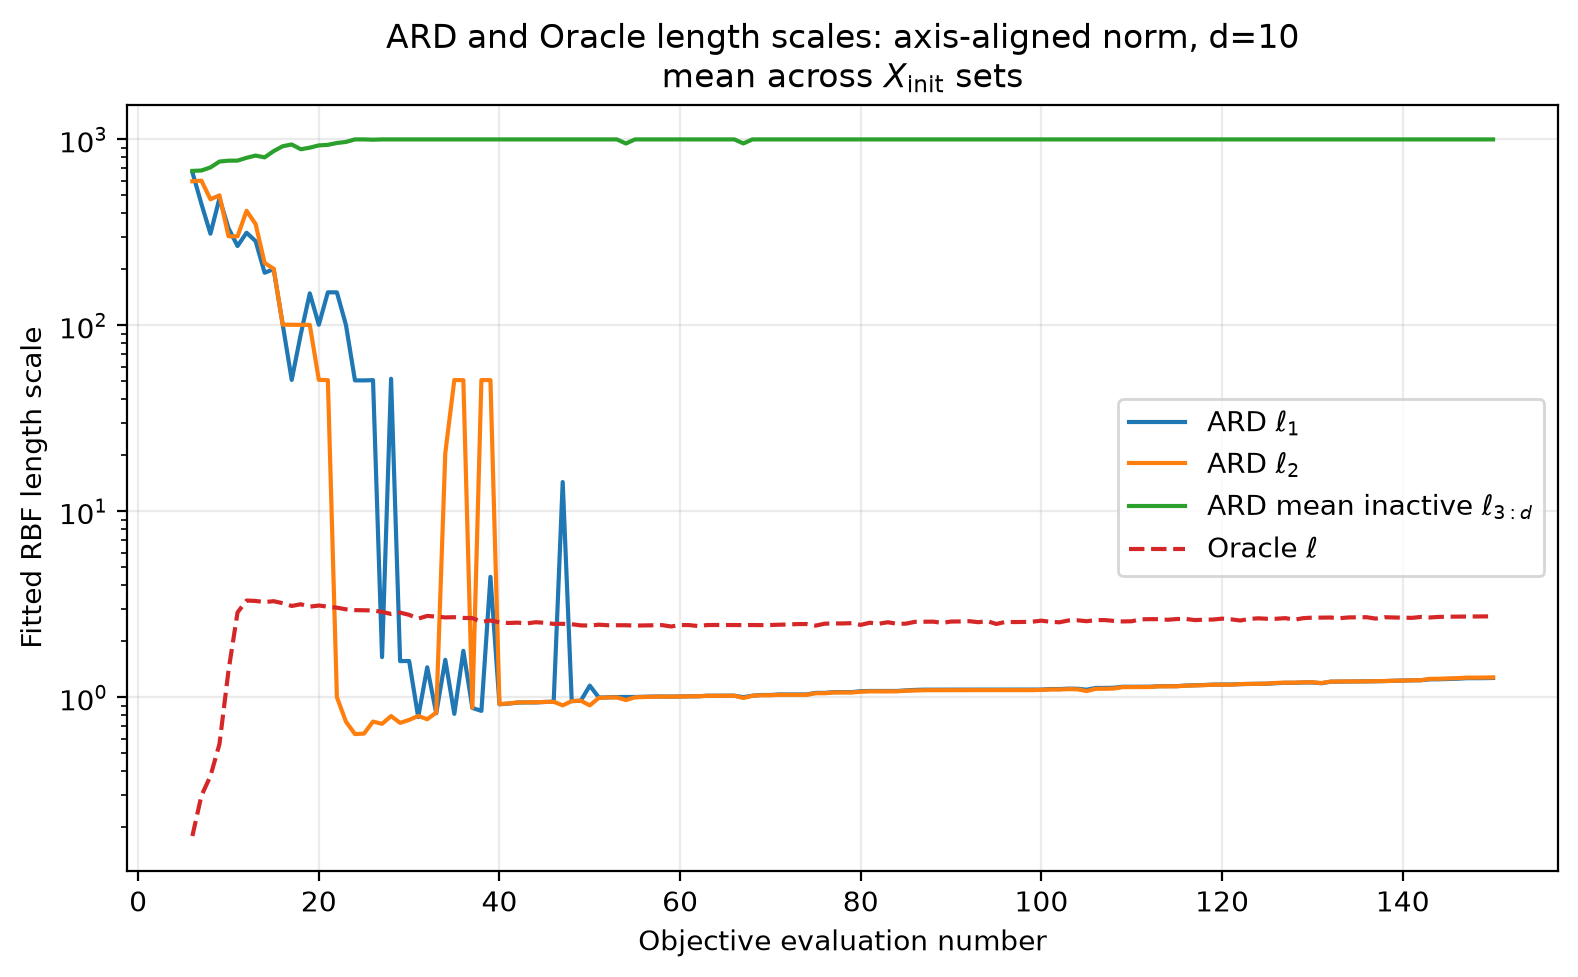
\includegraphics[width=\linewidth]
        {figures/diagnostics_ard_oracle/length_scales__d10.png}
        \caption{$d=10$}
        \label{fig:active-ls-d10}
    \end{subfigure}
    \hfill
    \begin{subfigure}[t]{0.48\textwidth}
        \centering
        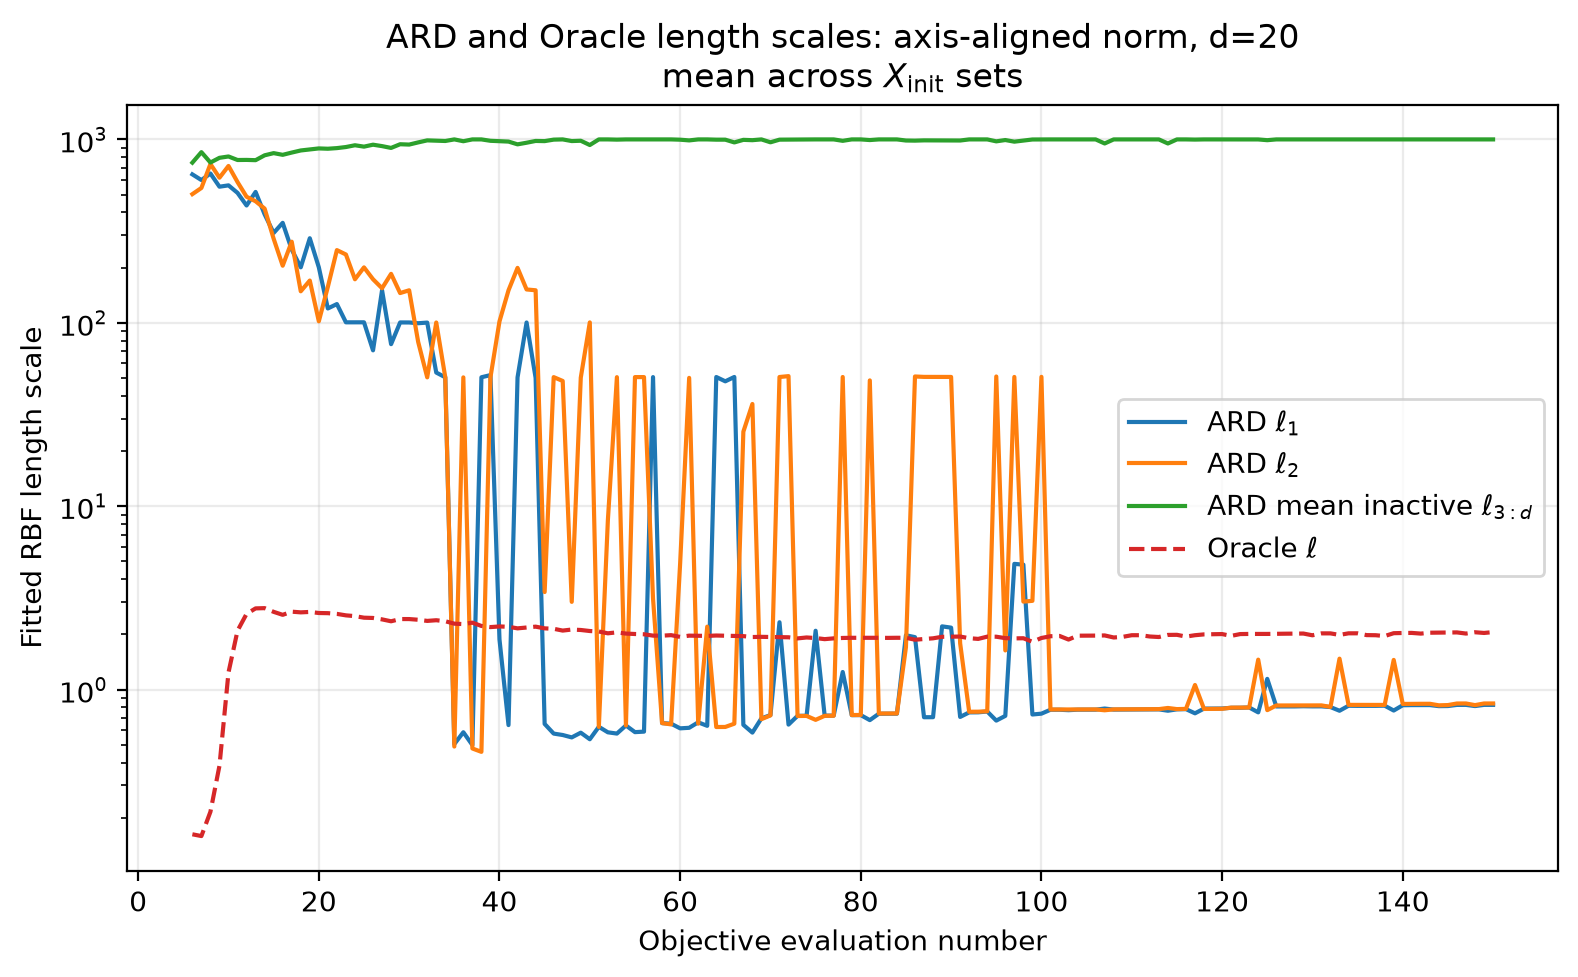
\includegraphics[width=\linewidth]
        {figures/diagnostics_ard_oracle/length_scales__d20.png}
        \caption{$d=20$}
        \label{fig:active-ls-d20}
    \end{subfigure}

    \caption{Fitted active-coordinate length scales for ARD-BO and Oracle BO on the axis-aligned norm objective across ambient dimensions.}
    \label{fig:ard-oracle-length-scales}
\end{figure}

\FloatBarrier

% === BIBLIOGRAPHY =====
% only if necessary. If your report does not cite any resource,
% which may very well be the case for this assignment, you 
% do not need to add a bibliography
%
%\clearpage
%\bibliographystyle{alpha}
%\bibliography{references}

\end{document}
